%%%%%%%%%%%%%%%%%%%%%%%%%%%%%%%%%%%%%%%%%
% Sullivan Business Report
% LaTeX Template
% Version 1.0 (May 5, 2022)
%
% This template originates from:
% https://www.LaTeXTemplates.com
%
% Author:
% Vel (vel@latextemplates.com)
%
% License:
% CC BY-NC-SA 4.0 (https://creativecommons.org/licenses/by-nc-sa/4.0/)
%
%%%%%%%%%%%%%%%%%%%%%%%%%%%%%%%%%%%%%%%%%

%----------------------------------------------------------------------------------------
%	CLASS, PACKAGES AND OTHER DOCUMENT CONFIGURATIONS
%----------------------------------------------------------------------------------------

\documentclass[
	a4paper, % Paper size, use either a4paper or letterpaper
	12pt,% Default font size, the template is designed to look good at 12pt so it's best not to change this
	%unnumberedsections, % Uncomment for no section numbering
]{CSSullivanBusinessReport}

\addbibresource{sample.bib} % BibLaTeX bibliography file

%----------------------------------------------------------------------------------------
%	REPORT INFORMATION
%----------------------------------------------------------------------------------------
\usepackage{siunitx}
\usepackage{amssymb}
\usepackage{xeCJK}
\usepackage{graphicx}
\usepackage{fontspec}
\usepackage{tikz}
\usepackage{geometry}
% \geometry{a4paper,right=2cm,top=1cm,bottom=1cm}

\reporttitle{Occidental Petroleum Corporation\texttrademark} % The report title to appear on the title page and page headers, do not create manual new lines here as this will carry over to page headers

\reportsubtitle{Business report and strategic analysis\\For SBL2 final assessment only} % Report subtitle, include new lines if needed

\reportauthors{\smallskip 黎子骏 \textit{20201504138}
\\\smallskip 李婷婷 \textit{20201503978}
\\\smallskip 许庭悦 \textit{20201504033}
\\\smallskip 叶炯尧 \textit{20201504251}
\\\smallskip 朱小天 \textit{20201504086}
} % Report authors/group/department, include new lines if needed
% 可以再次效仿格式填写个人信息
\reportdate{\today} % Report date, include new lines for additional information if needed

\rightheadercontent{
\includegraphics[width=3cm]{Images/zero_in.png}} % The content in the right header, you may want to add your own company logo or use your company/department name or leave this command empty for no right header content

%----------------------------------------------------------------------------------------
\bibliographystyle{ieeetr} 
\begin{document}
%----------------------------------------------------------------------------------------
%	TITLE PAGE
%----------------------------------------------------------------------------------------
% \usetikzlibrary{graphs, graphdrawing,positioning, calc, arrows.meta}
\thispagestyle{empty} % Suppress headers and footers on this page

\begin{fullwidth} % Use the whole page width
	\vspace*{-0.075\textheight} % Pull logo into the top margin
	
	\hfill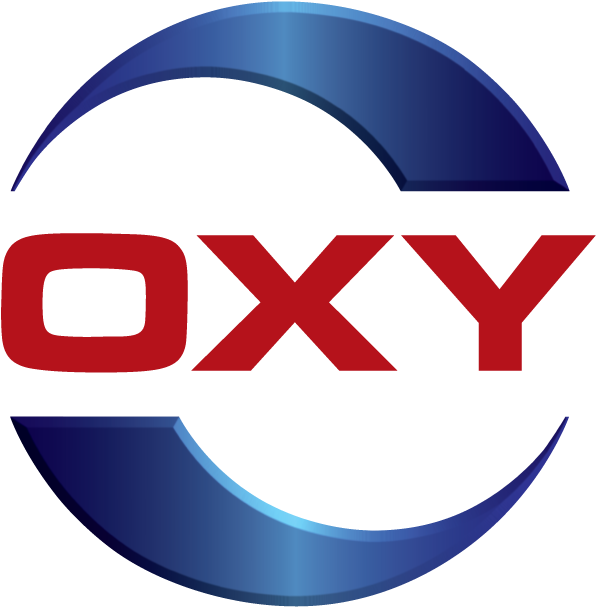
\includegraphics[width=5cm]{Images/OXY.png} % Company logo
	\vspace{0.15\textheight} % Vertical whitespace

	\parbox{0.9\fulltextwidth}{\fontsize{50pt}{52pt}\selectfont\raggedright\textbf{\reporttitle}\par} % Report title, intentionally at less than full width for nice wrapping. Adjust the width of the \parbox and the font size as needed for your title to look good.
	
	\vspace{0.03\textheight} % Vertical whitespace
	
	{\LARGE\textit{\textbf{\reportsubtitle}}\par} % Subtitle
	
	\vfill % Vertical whitespace
	
	{\Large\reportauthors\par} % Report authors, group or department
	
	\vfill\vfill\vfill % Vertical whitespace
	
	{\large\reportdate\par} % Report date
\end{fullwidth}

\newpage

%----------------------------------------------------------------------------------------
%	DISCLAIMER/COPYRIGHT PAGE
%----------------------------------------------------------------------------------------

\thispagestyle{empty} % Suppress headers and footers on this page

% \begin{twothirdswidth} % Content in this environment to be at two-thirds of the whole page width
	\footnotesize % Reduce font size
	
	\subsection*{Disclaimer}
    Please read the disclaimer carefully before reading the business report of OXY Co(“report”, "service") written by Kelp Li(黎子骏) and his fellow members("us","we","our").
\par
The content displayed on the website is the intellectual property of the us. You may not reuse, republish, or reprint such content without our written consent.
\par
The report format was programmed by Kelp Li. And the duty allocation, assignment guidance, report revision and editing works were done by Kelp Li.
\par
All information posted is merely for educational and informational purposes in SBL2 course in GDUFS. It is not intended as a substitute for professional advice. Should you decide to act upon any information on this website, you do so at your own risk.
\par
While the information in this report has been verified to the best of our abilities, we cannot guarantee that there are no mistakes or errors.
\par
We reserve the right to change this policy at any given time, of which you will be promptly updated. If you want to make sure that you are up to date with the latest changes, we advise you to feel free to contact us.
	
	\subsection*{Contact}
	
	GDUFS South campus, Higher education mega center, Panyu District, Guangzhou, Guangdong, PRC\\

	
	Post Code: 510420
	
	Contact: KelpLZJ@outlook.com / kelplzj@icloud.com;

	Source Code link:\url{http://github.com/KELP0122}
	
	\vfill % Push the following down to the bottom of the page
	
% 	\subsubsection*{Changelog}
	
% 	\scriptsize % Reduce font size further
	
% 	\begin{tabular}{@{} L{0.05\linewidth} L{0.15\linewidth} L{0.6\linewidth} @{}} % Column widths specified here, change as needed for your content
% 		\toprule
% 		v1.0 & 20XX-02-05 & Lorem ipsum dolor sit amet, consectetur adipiscing elit. Praesent porttitor arcu luctus, imperdiet urna iaculis, mattis eros.\\
% 		v1.1 & 20XX-02-27 & Pellentesque iaculis odio vel nisl ullamcorper, nec faucibus ipsum molestie.\\
% 		v1.2 & 20XX-03-15 & Sed dictum nisl non aliquet porttitor.\\
% 		\bottomrule
% 	\end{tabular}

% \end{twothirdswidth}

\newpage

%----------------------------------------------------------------------------------------
%	TABLE OF CONTENTS
%----------------------------------------------------------------------------------------

% \begin{twothirdswidth} % Content in this environment to be at two-thirds of the whole page width
	\tableofcontents % Output the table of contents, automatically generated from the section commands used in the document
% \end{twothirdswidth}

\newpage

%----------------------------------------------------------------------------------------
%	SECTIONS
%----------------------------------------------------------------------------------------
% \newgeometry{left=3cm,right=3cm}
\begin{fullwidth}
    
\section{(黎子骏) Introduction} % Top level section

\subsection{Abstract}
The report analyzes the operation and strategy of Occidental Petroleum from both the external and internal level.
gives assessment on the past operating performance.
\par
The report will first have a brief overview of Occidental Petroleum's background corporate culture, and political tendency, and then focus on the social political environment of Occidental Petroleum Corporation, including the nature of oil industry in the United States, the transformation of national strategy and national economy, and recent news.
\par
The remaining parts of the report are to be organized as followed: The 2nd part is External Analysis, where further and deeper assessment on external environment will be presented.  
The 3rd section is the SWOT analysis. 
The 4th section is the Financial Analysis, where this report assess the past performance and evaluate the influence of recent M\&A case. 
The 5th section is Business Level analysis, where we figure the three strategies of Occidental Petroleum: Cost leadership, Differentiation and Focus.
The last section is conclusions and recommendations.

\subsection{Brief overview of Occidental Petroleum Corporation}
\subsubsection{Background about OXY}

Occidental’s principal businesses consist of three reporting segments: oil and gas, chemical and midstream and
marketing. The oil and gas segment explores for, develops and produces oil (which includes condensate), natural gas
liquids (NGL) and natural gas. The chemical segment (OxyChem) primarily manufactures and markets basic chemicals and
vinyls. The midstream and marketing segment purchases, markets, gathers, processes, transports and stores oil (which
includes condensate), NGL, natural gas, carbon dioxide (CO2) and power. It also optimizes its transportation and storage
capacity, and invests in entities that conduct similar activities, such as Western Midstream Partners, L.P. (WES).
\par
The midstream and marketing segment also includes Occidental’s low carbon ventures (OLCV) businesses. OLCV
seeks to leverage Occidental’s legacy of carbon management expertise to develop carbon capture, utilization and storage
(CCUS) projects, including the commercialization of direct air capture (DAC) technology, and invests in other low-carbon
technologies intended to reduce greenhouse gas (GHG) emissions from our operations and strategically partner with other
industries to help reduce their emissions.\cite{AnnualRepo2021}

\subsection{Human capital resources and corporate social responsibility}
Corporate culture is one of the key factors that determine the corporate governance.\cite{LU2021101264}  And the companies in countries that are of low power distance, individualism, femininity and long-term orientation tend to disclose more about corporate social responsibility (CSR).\cite{SUN2020101256} Hence analyzing the human capital resources and CSR disclosures may help understanding the social-cultural  aspect of the business environment in the USA. According to the 2022 annual report, the culture of Occidental petroleum are:\cite{CodeOfConduct}
\begin{itemize}
    \item Lead with passion
    \item Outperform Expectations
    \item Deliver result responsibly
    \item Outperform Expectations
    \item Commit to good
\end{itemize}
And the report uses 3 paragraphs to describe the diversity, inclusion AND belongings. During the first quarter of 2021, Occidental established the DIB Advisory Board and the DIB Ambassador Committee. Such action complies with the multi-culture environment in the USA and therefore may promise a brighter development outlook.
\par
Further analysis will be presented in the "Corporate-level" section.

\begin{figure}[h]
    \centering
    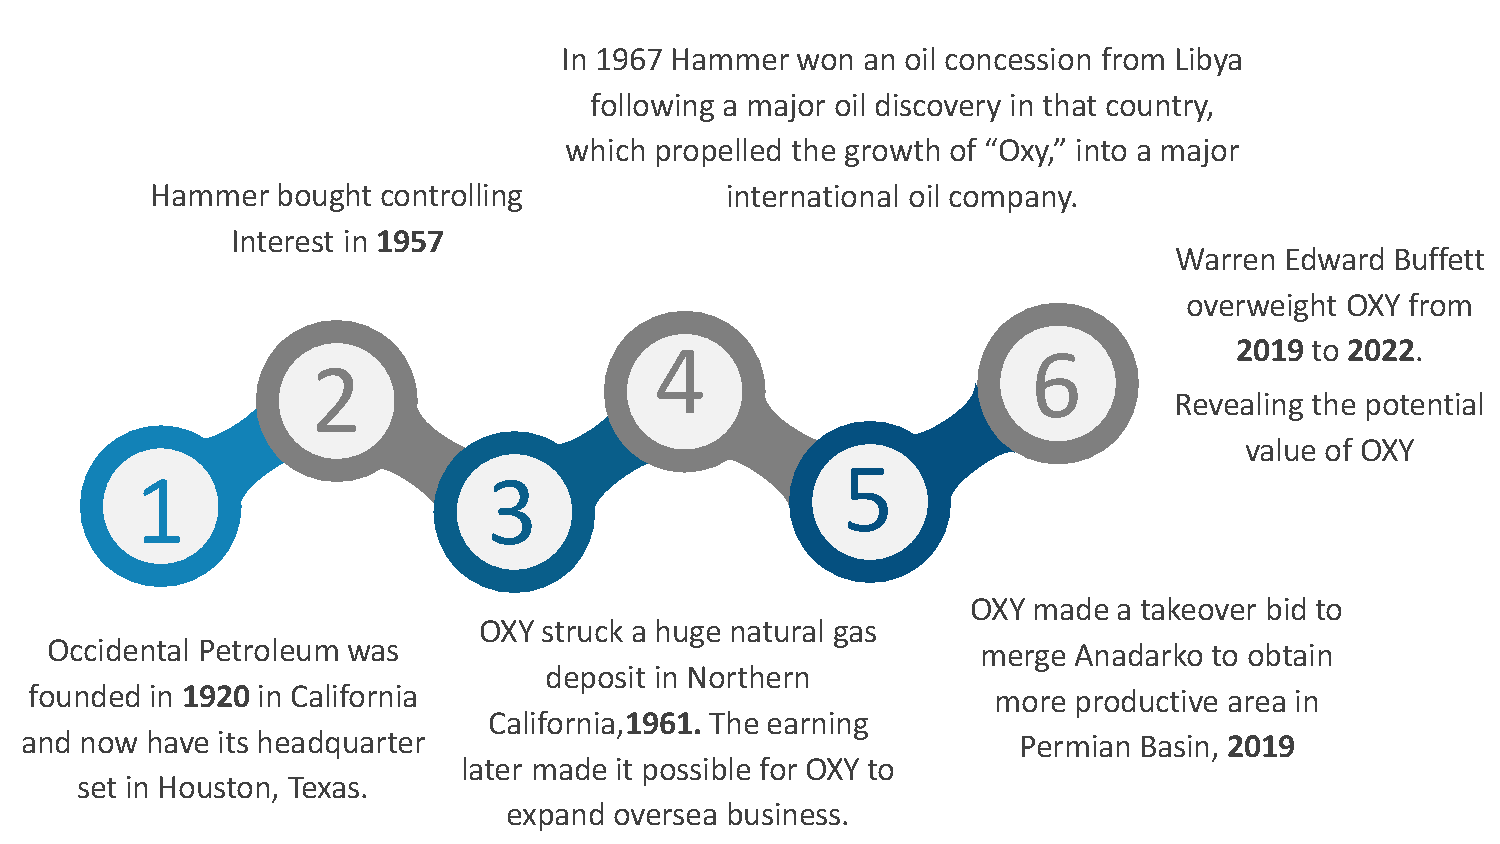
\includegraphics[width=18cm]{Images/chronicle.pdf}
    \caption{The chronicle of OXY Co}
    \label{chronicle}
\end{figure}
\par


\subsubsection{Recent News}

On August 8, 2019, pursuant to the Agreement and Plan of Merger dated May 9, 2019, Occidental acquired all of the
outstanding shares of Anadarko Petroleum Corporation (Anadarko), through a transaction in which a wholly owned
subsidiary of Occidental merged with and into Anadarko (the Acquisition). The Acquisition added to Occidental's oil and gas
portfolio, primarily in the Permian Basin, DJ Basin, Gulf of Mexico and Algeria, and an interest in WES.

The takeover bid of Anadarko in 2019, which was supported by finance giant Warren Buffet, has brought heavy debt burden to OXY Co. There have been arguments over this matter even until today.
Although the financial status OXY is still quite robust. The risk of going cocern problems has increased with the rise of debt gearing. 
Modigliani and Miller (1963) recognized the tax-shield effect of debt finance in the corporate capital structure.\cite{10.2307/1809167} Theoretically, the higher the gearing is, the lower the after-tax weighted average cost of capital will be. However,in reality there are more to consider. 
\par
The agency cost is one of the factor that may exert influence on the financial analysis of OXY Co. The agency cost is defined as the generic term of all kinds of cost generated as a result of the principle-agent relationship\cite{ross1973} When the company has debt burden, there will be conflicts between shareholder and creditor. The conflict could have been more fierce in financial distress, and eventually increase the agency cost for the company. Above all, the existence of debt burden may motivate shareholder to seek 3 kinds of strategy that may damage the interest of creditors.\cite{Ross1977}
\begin{enumerate}
    \item \textbf{Incentives to take high risk.} Especially for the companies that have going-concern problems.
    \item \textbf{Insufficient investments.} Shareholders of the companies that are of high bankrupt risk often find that news investments will end up compensating creditors by sacrificing the interest of shareholders, and hence lead to lack of investments.
    \item \textbf{Pay extra dividends or other distribution projects.} The retained earnings for creditors will be less.
    
\end{enumerate}
The debt gearing level can also be a signal to investors. Only those successful enterprises will take high debt gearing. \cite{incentivesignalling}.

\par
Besides, this report had done due diligence investigation of the political postiion of Vicki Hollub, who is serving as the CEO of OXY Co. Table \ref{dd} shows that most of the contributions ard paid to red politicians, or the republicans. So this may a potentioal political threat during the tenure of President Joe Biden, comparing with other blue companies.
\begin{table}[!ht]\footnotesize
    \centering
    \caption{The senior board members of Occidental Petroleum}
    \begin{tabular}{ll}
    \hline
        Name & Title  \\ \hline
        Vicki Hollub & PRESIDENT AND CHIEF EXECUTIVE OFFICER  \\ 
        Marcia E. Backus & Senior Vice President, General Counsel and Chief Compliance Officer  \\ 
        Robert L. Peterson & Senior Vice President and Chief Financial Officer  \\ 
        Richard A. Jackson & President, Operations, Onshore Resources and Carbon Management  \\ 
        Kenneth Dillon  &  President, International Oil and Gas Operations  \\ 
        Peter J. Bennett  &  President, Development, Onshore Resources and Carbon Management  \\ 
        Neil R. Ackerman  &  President, Occidental Chemical Corporation  \\ 
        Jeff F. Simmons  &  Senior Vice President, Technical and Operations Support \& CPTO  \\ 
        Sunil Mathew  &  Vice President, Strategic Planning and Analysis and Business Development  \\ 
        Frederick A. Forthuber  &  President, Oxy Energy Services  \\ 
        Charles F. Weiss  &  Senior Vice President, Environmental and Sustainability  \\ \hline
        \\Data source: 2022 annual report
    \end{tabular}

\end{table}

\begin{table}[h]\small
    \centering
    \caption{Political contribution paid by Vicki Hollub}
    \begin{tabular}{lll}
    \hline
        Recipient & Amount \$ & Times \\ \hline
       \textbf{ Money to Candidates} & 75181 & 49 \\ 
        \textbf{{CO}} & \textbf{1100} & \textbf{1} \\ 
        \quad HICKENLOOPER, JOHN W \& GARCIA, JOSEPH (JOE) (D) & 1100 & 1 \\ 
        \quad Federal & 13400 & 6 \\ 
        \quad Heidi Heitkamp (D) & 7900 & 4 \\ 
        \quad Kevin McCarthy (R) & 2700 & 1 \\ 
        \quad Mitch McConnell (R) & 2800 & 1 \\ 
        \textbf{{TX}} & \textbf{35681} & \textbf{41} \\ 
        \quad CHRISTIAN, WALTER W (WAYNE) (R) & 5000 & 1 \\ 
        \quad CRADDICK, CHRISTI (R) & 12500 & 2 \\ 
        \quad OCCIDENTIAL PETROLEUM & 13181 & 37 \\ 
        \quad SITTON, RYAN (R) & 5000 & 1 \\ 
        \textbf{VA} & \textbf{25000} & \textbf{1} \\ 
        \quad ED GILLESPIE CAMPAIGN CMTE (R) & 25000 & 1 \\ 
        \textbf{Money to PACs} & \textbf{28028} & \textbf{50} \\ 
        \quad Federal & 28028 & 50 \\ 
        \quad Great America Cmte (R) & 5000 & 1 \\ 
        \quad Lockheed Martin & 6500 & 7 \\ 
        \quad Occidental Petroleum & 16528 & 42 \\ 
        \textbf{Money to Parties} & \textbf{12300} & \textbf{1} \\ 
        \quad Federal & 12300 & 1 \\ 
        \quad National Republican Congressional Cmte (R) & 12300 & 1 \\ 
        \textbf{Sum} & \textbf{115509} & \textbf{100} \\ \hline
        Datasource: The U.S Federal Election Committee.\cite{politicalcon}. \\
        The corporate level data can be found in appendices.
    \end{tabular}
    
    \label{dd}
\end{table}
Further financial analyses are to be presented in the "financial analysis" section.
\subsection{The nature of the oil industry}
    The oil business is different from the ones of other commodities. For oil has been serving as not only a product in the commodity market, but also a strategic resource for national strategy. Hence international political factors will interfere with the market operation. \par

    \begin{figure}[H]
        \centering
        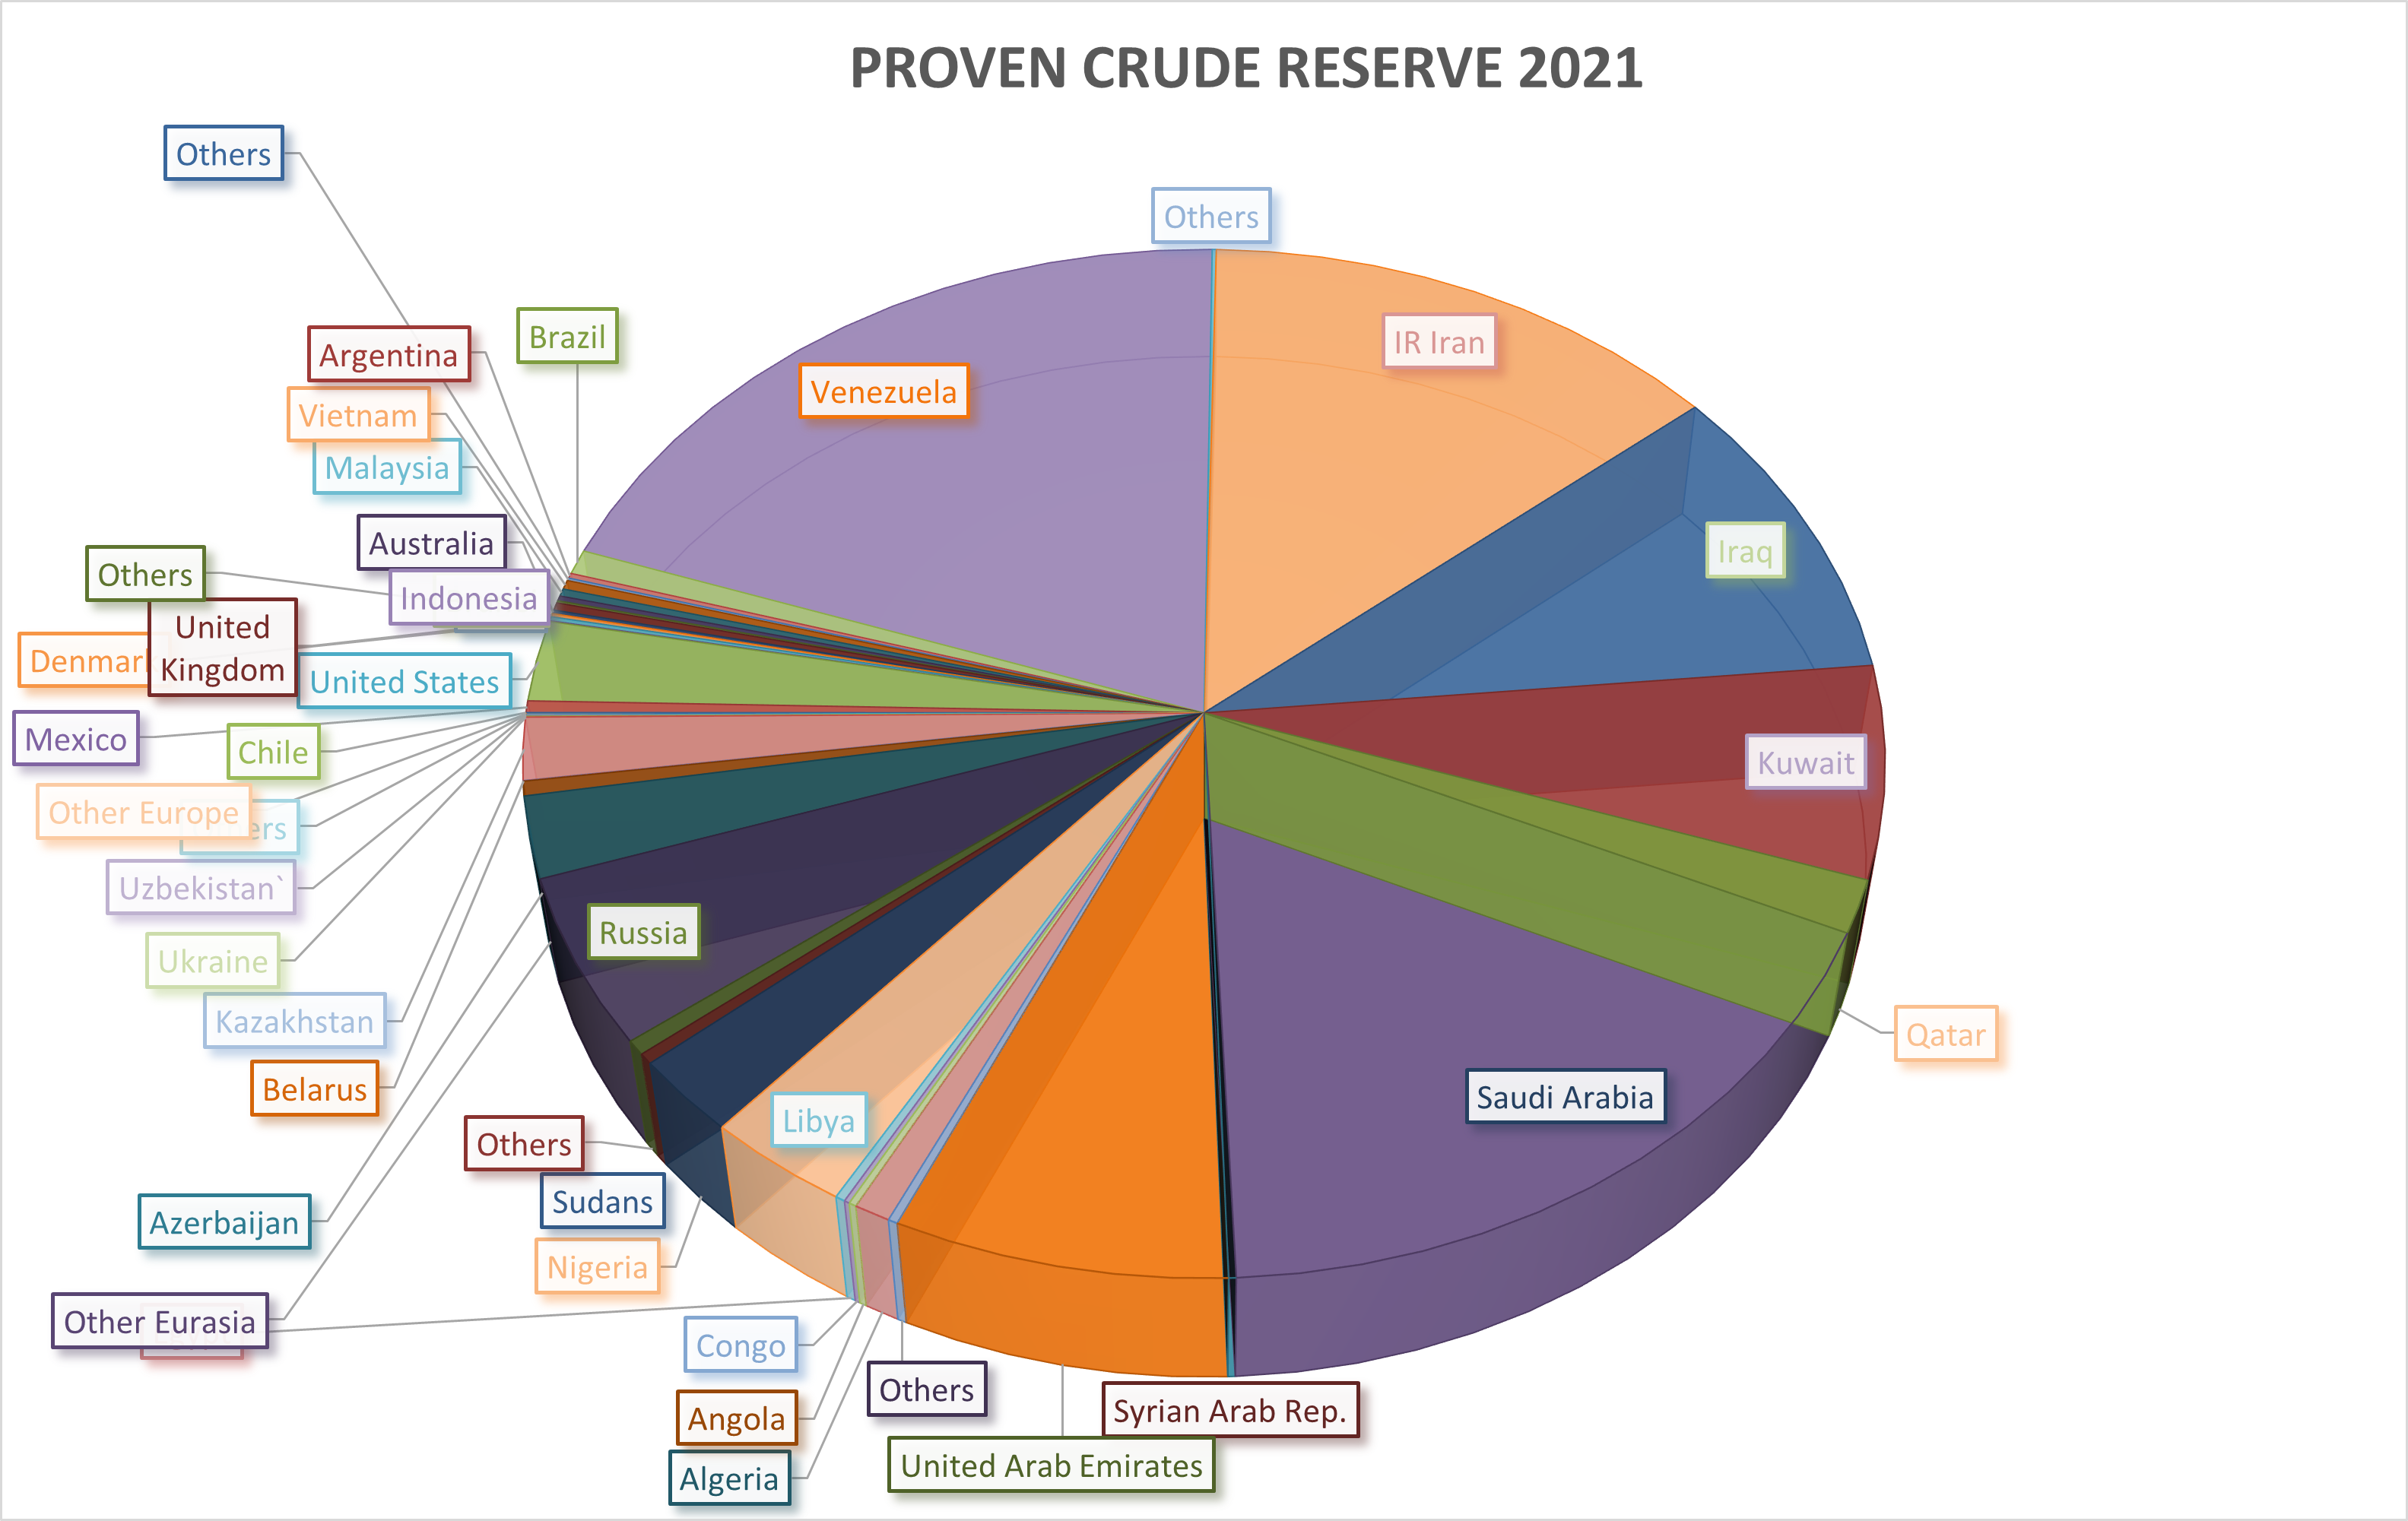
\includegraphics[width = 10cm]{Images/Proven Crude Reserve 2021.png}
        \caption{Proven Crude Reserve in 2021}
        \label{crude2021}
    \end{figure}
    
    \begin{figure}[H]
        \centering
        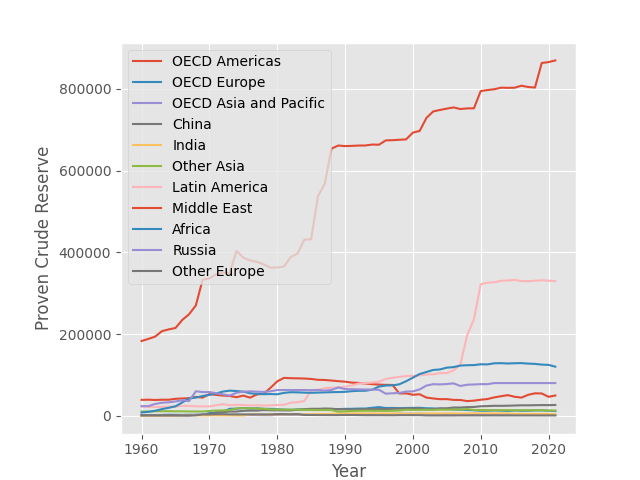
\includegraphics[width = 10cm]{Images/crude_reserve.png}
        \caption{Proven reserve 1960-2021 Unit: 10k barrels}
        \label{panelreserve}
    \end{figure}
    \par
    Oil companies' performance will be influenced from 4 dimensions:
    \begin{itemize}
        \item Demand:
\begin{itemize}
    \item The demand elasticity of oil is quite small, and oil is a typical kind of rigid demand. Although there had been voices that oil will be replaced by renewable energy in the future, the market share of oil and the significance in national defense ensure the long-lasting demand for oil.
\end{itemize}
        \item Supply:
\begin{itemize}
    \item Due to the exogeneity of the oil reserve, the market is commonly defined as oligopoly. As  figure \ref{crude2021} and \ref{panelreserve} shown, most of the world's oil reserve is controlled by OPEC countries, the United States and Russia.
    \end{itemize}
    \item Price:
        \begin{itemize}
        \item The price are internationally unified and the pricing rights are in the hands of oligarchies. Usually the oil prices are globally unified, however, in countries like China, the oil prices can be different from international oil price.
        \item The S\&P Oil index measures the performance of the top 120 listed oil companies worldwide. According to figure \ref{SPindex}, the curve of oil price and S\&P index are quite fit in shape. So the oil company's performance and oil prices can be recognized as related.
        \begin{figure}[H]
            \centering
            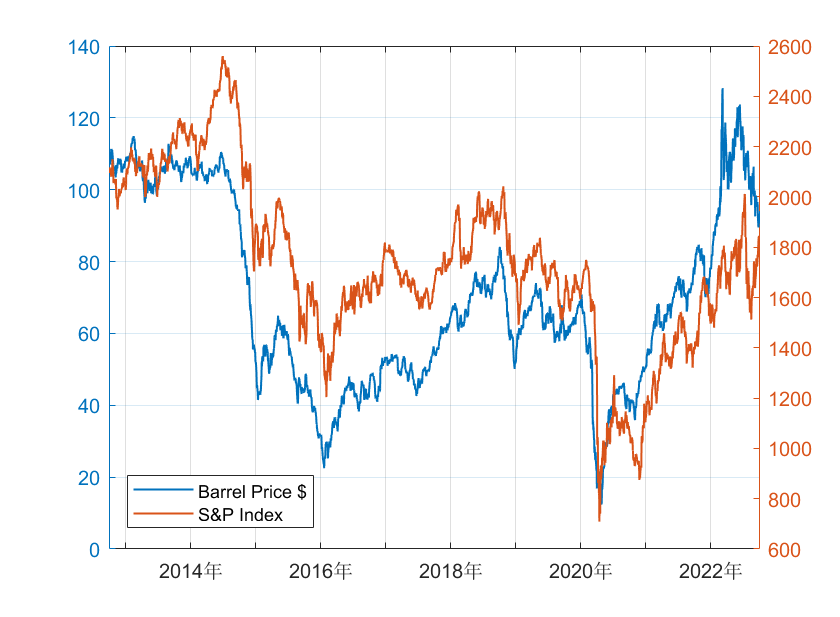
\includegraphics[width=10cm]{Images/doubleYoil.png}
            \caption{The S\&P index and oil price}
            \label{SPindex}
        \end{figure}
        \end{itemize}
    \item Determinants: 
        \begin{itemize}
        \item The global social-political power will influence the operation of oil companies. For example, the US president election will determine the fate of oil companies that supports the counterpart in the following tenure.
        \end{itemize}
    \end{itemize}

\subsection{The Review of fossil Industry in the United States} 
The United States has been extracting oil since the 1850s and in the years since increased oil production to over 16 million barrels per day.
\par
Texas is the leading oil-producing state in the country. The Permian basin and Eagle Ford Shale Play are largely located in Texas and one of the most actively drilled targets for conventional and unconventional oil, such as shale and oil sands. Due to the coronavirus pandemic, the number of operational oil rigs in the U.S. was significantly reduced in 2020, but has since been on the way to recovery. Although the Permian basin is the most productive oil region, the neighboring Eagle Ford play and North Dakota’s Bakken Formation ranked first in terms of oil production per new well. \par
As for oil industry, the crude reserve in the US was never comparable with the ones in the Middle East and Latin America. Since the discovery of the shale oil reserve in the US mainland, the influence of US in the supply side has become more powerful. \par
Up until the past decade, the majority of crude oil withdrawn in the U.S. was taken from carbonate and sandstone reservoirs as a result of the shale oil revolution in 21th century. This liquid fossil fuel is found both in reservoir rocks and source rocks, with the latter having become more accessible and financially viable following technological advances. The U.S. holds the world’s ninth-largest oil reserves worldwide.

\subsection{The transformation of the US strategy and economy}
Offshoring has been a hallmark of US firms’ manufacturing strategy, on account of its beneficial effects in terms of costs and access to new markets.\cite{DIMAURO2022102006}
Back-shoring is defined as moving business back from abroad to home.\cite{backshoring}. The back-shoring trend has occurred after decades of off-shoring in the US manufacturing industry and entered into climax since Donald Trump's first tenure. The slogan raised by republicans:"MAGA", whcih stands for "Making America Great Again", has greatly stimulated the foreign investment to back-shore. 
\par
The core idea of the right wing strategy is deglobalization. For the United States, the powerful manufacturing industry had been the pearl on the crown of Statue of Liberty. However, with the rising labor cost in the US mainland, many corporations in the secondary industry chose the off-shoring path of operation. But due to international geopolitical reason and the change in the national strategy of Fedral governments, the US authorities are expecting oversea secondary enterprises to back-shore to mainland so as to gain advantage in the gaming with China and Russia. Oil, as the blood for industry, has always been the core strategic resource of the United States. As the Chinese saying goes,"Food and fodder should go ahead of troops and horses.
". The back-shoring of oil giants has been attached with great importance with the United States. The back-shoring trend is especially significant in "red" companies like OXY Co as this report has analyzed above. The result may be reflected in the focus strategy in the "Business-level" section.
\par
However, during the current tenure of President Joe Biden and his democrats cabinet may promote renewable energy in the civilian transportation, which may damage the market share of OXY Co for the future demand for fossil energy in daily transportation may fad with the lapse of time. It also worths considering that the consumption habit in the United States matters. The typical stereotype for US lifestyle is high-carbon emission: Driving cars with larger gas displacement, consuming a lot of meat, wasting food and electricity an so on. The key contradiction is whether the left-wing democrats like Joe Biden can change American people's lifestyle or not. The result may determine the future domestic market for Occidental Petroleum.

\section{(朱小天)External Analysis}
\subsection{PESTEL Analysis}
OXY is a typical crude petroleum \& natural gas company in the upstream of the industry, and the price of crude oil and natural gas directly affects the company's earnings and strategic adjustment. However, the impact of macro environment on crude oil and natural gas price is direct and significant. To some extent, the PESTEL analysis of crude oil price and natural gas is also the analysis of OXY Company, so the PESTEL analysis is not only for the company itself, but also for crude oil and natural gas price.
\begin{figure}[h]
    \centering
    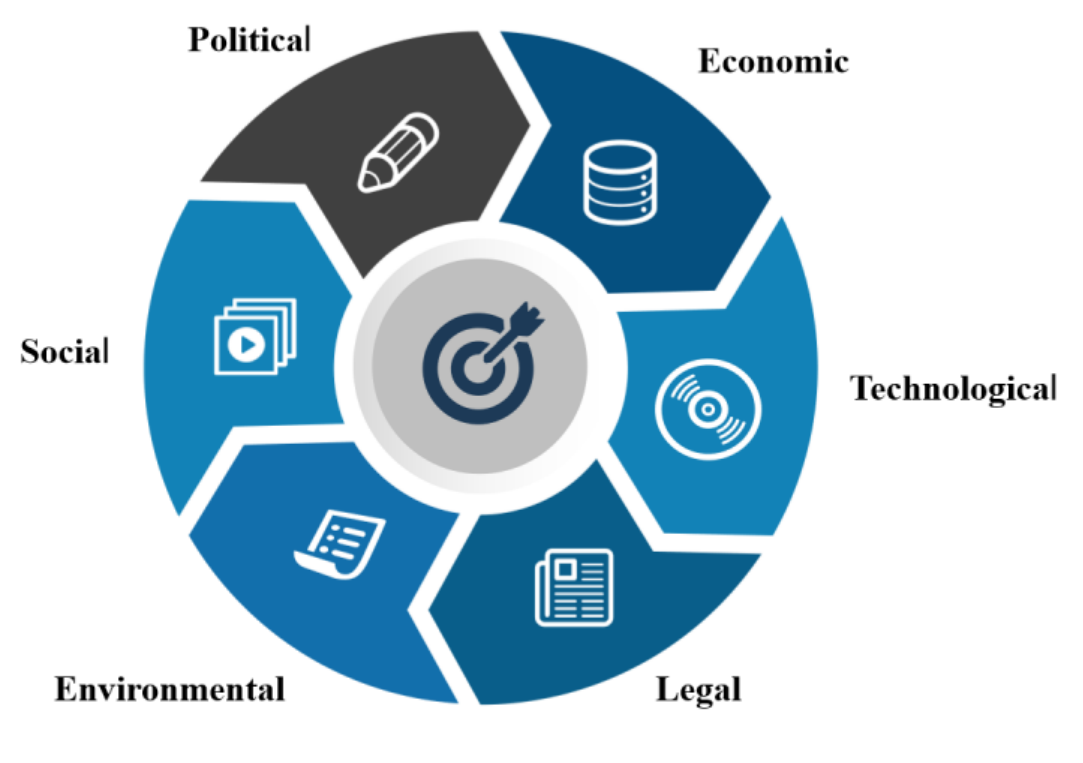
\includegraphics[width=10cm]{Images/PESTEL.png}
    \caption{PESTEL Model}
    \label{pestel}
\end{figure}
Detailed Analysis
\par

\subsubsection{Political}
\begin{enumerate}
    \item \textbf{Global factors}
\par
There are two forces, OPEC and big oligopolies in the United States. OPEC are traditional crude oil pricing organization(like a cartel) and are affected by geopolitical risks. 
\par
The Organization of the Petroleum Exporting Countries is a cartel of 13 countries. Founded on 14 September 1960 in Baghdad by the first five members. As of September 2018, the 13 member countries accounted for an estimated 44 percent of global oil production and 81.5 percent of the world's proven oil reserves, giving OPEC a major influence on global oil prices that were previously determined by the so-called "Seven Sisters" grouping of multinational oil companies.  However, as the U.S. pumps more petroleum for the reasons of technologies revolution, pricing power gradually shifts to the U.S. petroleum oligopolies.
\par
Recently, Russia-Ukrain War leads to the rising price and uncertainty of petroleum.The war and Western sanctions against Russia have resulted in a sharp decrease in the flow of crude oil and natural gas from Russia into the international market, leading to the rise and uncertainty of international oil prices.

\item \textbf{Domestic factors in United States}
\par
US Democrats have been pushing for shifts to clean energy which is the substitute of petroleum. When U.S. President Joe Biden was running for the Democratic presidential nomination, the Biden’s team issued Plan for Clean Energy Revolution and Environmental justice. Democrats’ target is to ensure that the United States has a 100\% clean energy economy and achieves net zero carbon emissions by 2050. Their solutions are as follows. Firstly, the federal government's procurement system will spend \$500 billion a year to achieve 100\% clean energy and zero vehicle emissions. Secondly, the federal government will develop more stringent new fuel emissions standards to ensure that 100\% of newly sold light or medium vehicles are electric. Thirdly, Mr.Biden will announce his reentry into the Paris Agreement on his first day in office.
As the substitute of petroleum, clean energy’s development is a threat to petroleum industry.

\end{enumerate}

\par

\subsubsection{Economic}
Global economic conditions will affect international crude oil prices, as will domestic economic conditions in the United States. There is interaction between inflation and the rising of crude oil prices. Inflation in the United States has led to soaring prices , which has led to a rise in domestic oil prices.
\par
The global economic downturn caused by the COVID-19 pandemic has reduced demand for oil in general. Many industries have been shut down because of COVID-19. Transportation has been halted and many air routes have been suspended. These all result in lower demand for oil. Meanwhile, the economic recovery of some regions and countries have increased the demand for petroleum and made the oil price tend to rebound.
\par
To sum up, the market supply and demand relationship caused by the economic environment is complex, so the impact of the economic environment on the oil price is also complex and comprehensive. It is difficult to generalize.
\subsubsection{Social}
The awareness of environmental protection in the whole society has been significantly increased. People's acceptance of new energy vehicles has greatly improved. Social consumers’ interest in new energy vehicles is increasing. According to a survey from Consumer Reports on electric cars, a whopping 71\% of US drivers say they would consider buying an electric vehicle at some point in the future. As the substitute of fossil-fueled cars, new energy vehicle’s development and improved acceptance are a threat to fossil-fueled cars.
\par
A number of environmental groups and environmental demonstrations have sprung up in society, among which the representative figure is the Swedish environmental activist Greta Thunberg. These environmental organizations and demonstrations will contribute to a wide range of environmental trends in the society.
\subsubsection{Technological}
As the development and wide application of fracking, American oil production has taken a qualitative leap and can be able to compete with OPEC. The success of the shale gas and oil revolution in the United States has led to it being the only country in the world to commercially extract shale oil and gas resources. Fracking is a proven drilling technology used for extracting oil, natural gas, geothermal energy, or water from deep underground. Fracking has been safely used in the United States since 1947. More than 1.7 million U.S. wells have been completed using the fracking process, producing more than seven billion barrels of oil and 600 trillion cubic feet of natural gas.
\par
The development of new energy vehicles (NEVs) and battery-related technologies will make the market tend to choose new energy rather than traditional petroleum energy. NEVs mainly refer to pure battery electric vehicles (BEV), plug-in electric vehicles (PHEV) and fuel cell vehicles (FCEVs).
\subsubsection{Environmental}
The global need for environmental protection and low carbon emissions is urgent. Paris Agreement is a representative example. Climate change is a global emergency that goes beyond national borders. It is an issue that requires international cooperation and coordinated solutions at all levels. To tackle climate change and its negative impacts, world leaders at the UN Climate Change Conference in Paris reached a breakthrough on 12 December 2015: the historic Paris Agreement. Paris Agreement is a landmark agreement that brought environmental awareness to a global level.
\par
The oil production industry is constrained by geography and the discovery of new fields. If a new oil field is discovered and used by OXY, the value added to the company will be huge.
\subsubsection{Legal}
The legality of oil exploration rights in specific lands.
\par
The ownership of oil and gas rights in the United States differs from most international jurisdictions in that a significant portion of oil and gas rights are privately held by individuals  and can be transferred freely between private parties. The federal government owns and controls oil and gas rights on US-owned lands, which cover large portions of the country, around 28\% of all onshore lands located in the United States, and include land located within individual states’ geographic boundaries. On state-owned lands within the geographic boundaries of the applicable state, oil and gas rights are owned by the individual states. States with a coastline own the oil and gas rights to any submerged lands up to three nautical miles from their coastlines except Texas and Florida, which own the rights up to three marine leagues from the coastline. The federal government owns the oil and gas rights to any US submerged lands beyond such state-controlled lands, including on the outer continental shelf. (Source:Oil and gas exploration and production laws in the USA, Morgan, Lewis & Bockius LLP)
\par
Oil and gas concessions are the lifeblood of oil companies, especially those like OXY that are upstream in the petroleum industry. However, the exploitation right is owned by the government, which indicates that OXY is restrained by the law and the government to some extent.
\subsection{Porter’s five forces model}
\begin{figure}
    \centering
    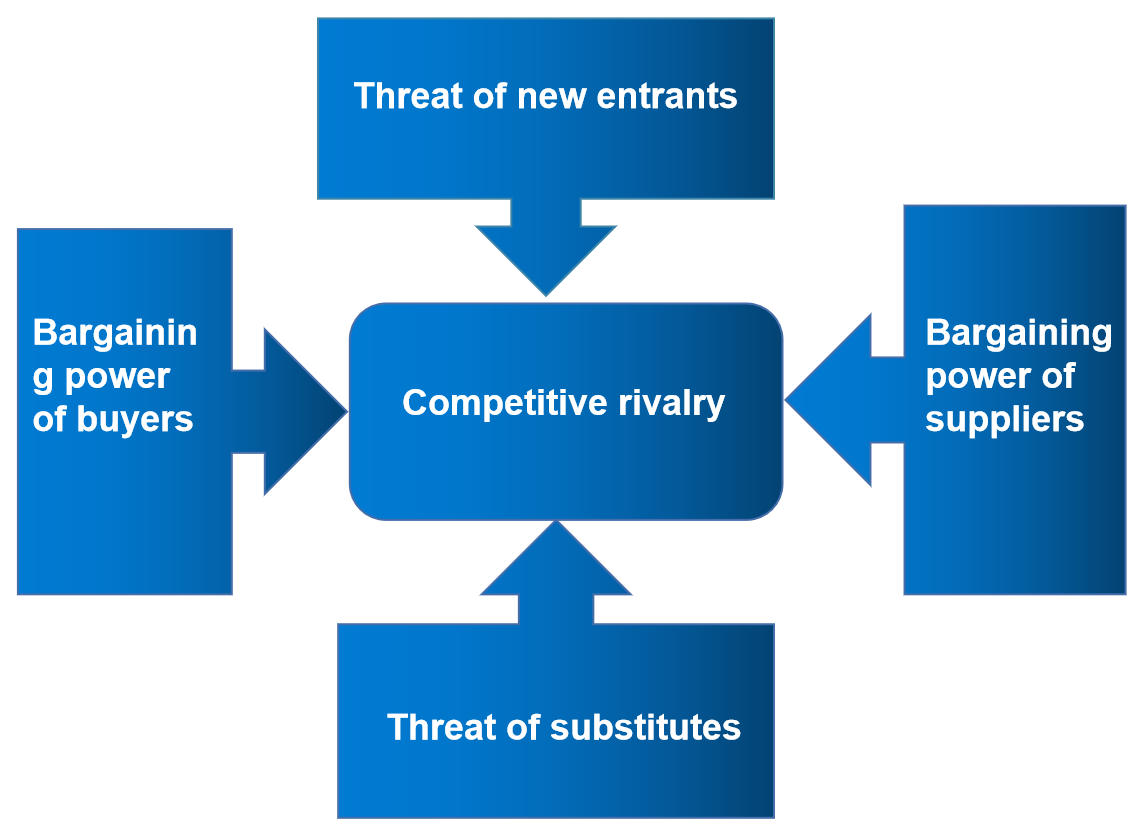
\includegraphics[width=10cm]{Images/Five forces.png}
    \caption{Porter's five forces model}
    \label{five forces}
\end{figure}
\subsubsection{Bargaining power of suppliers} 
Bargaining power of suppliers is low in general. OXY itself is one of the suppliers of crude oil in USA. Manufacturers of specially constructed tools and machinery to extract oil fields.
\subsubsection{Threat of new entrants}
Threat of new entrants is not a problem. Crude oil is the scarce resource. Its exploitation is limited by geography, exploration legal rights and technology. The accumulation of oil fields is very limited. Therefore,the barriers to entry are particularly high.
\subsubsection{Bargaining power of buyers}
Bargaining power of buyers is low. Crude oil is a scarce resource and is known as "the blood of industry". Although the new energy industry is booming, it is undeniable that oil will still be the essential resource for the global industry for a long time.\par
Oil pricing is cartel pricing, and there is little difference in crude oil prices between different petroleum companies. However, the demand elasticity of oil is very small, which leads to low bargaining power of buyers.
\subsubsection{Threat of substitutes}
Threat of substitutes is significantly powerful. The share of oil consumed by road globally reaches approximately 50\%. The rise of the new energy automobile industry has undoubtedly had a significant impact on the fossil-fuelled cars industry. The demand for fuel has been greatly reduced, and the blow to the oil industry is also huge.(“OECD” in the following image refers to Organization for Economic Co-operation and Development.)
\begin{figure}
    \centering
    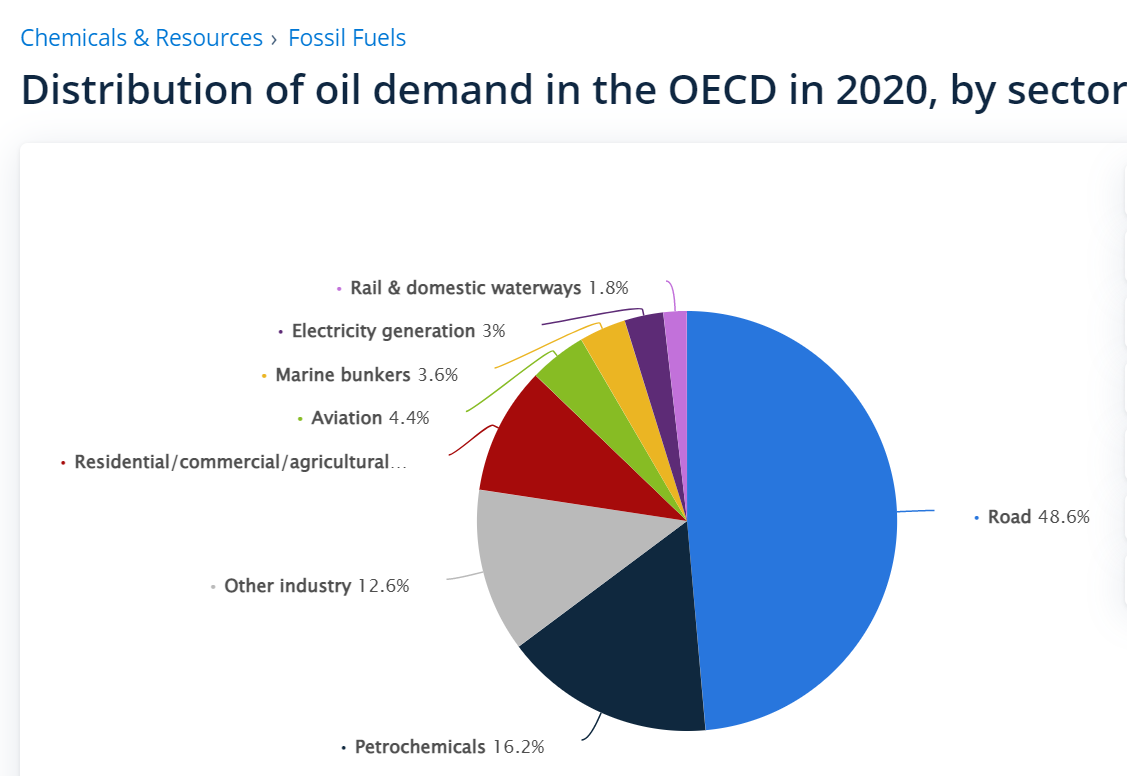
\includegraphics[width=10cm]{Images/Threat of substitute.png}
    \caption{Distribution of oil demand in the OECD in 2020}
    \label{Distribution of oil demand in the OECD in 2020}
\end{figure}
\subsubsection{Competitive rivalry}
There are several brands in the market which are competing for the same set of customers. According to annual report 2021 of OXY, Occidental’s peer group consists of BP p.l.c., Chevron Corporation, ConocoPhillips, EOG Resources, Inc., ExxonMobil Corporation, Shell, TotalEnergies SE (Total) and Occidental.
Meanwhile, the main competitors of Occidental Petroleum include Petróleo Brasileiro S.A. - Petrobras (PBR), Pioneer Natural Resources (PXD), Canadian Natural Resources (CNQ), ENI (E), EOG Resources (EOG), Devon Energy (DVN), Cenovus Energy (CVE), Continental Resources (CLR), Diamondback Energy (FANG), and Woodside Energy Group (WDS). These companies are all part of the "crude petroleum & natural gas" industry. (Source: marketbeat.com)\par
However, in view of the fact that oil is a scarce resource, it is not in a perfectly competitive market, so its relationship with competitors and the way it competes is different from that of an industry in a perfectly competitive market.
\subsection{SWOT Analysis}
\begin{figure}[h]
    \centering
    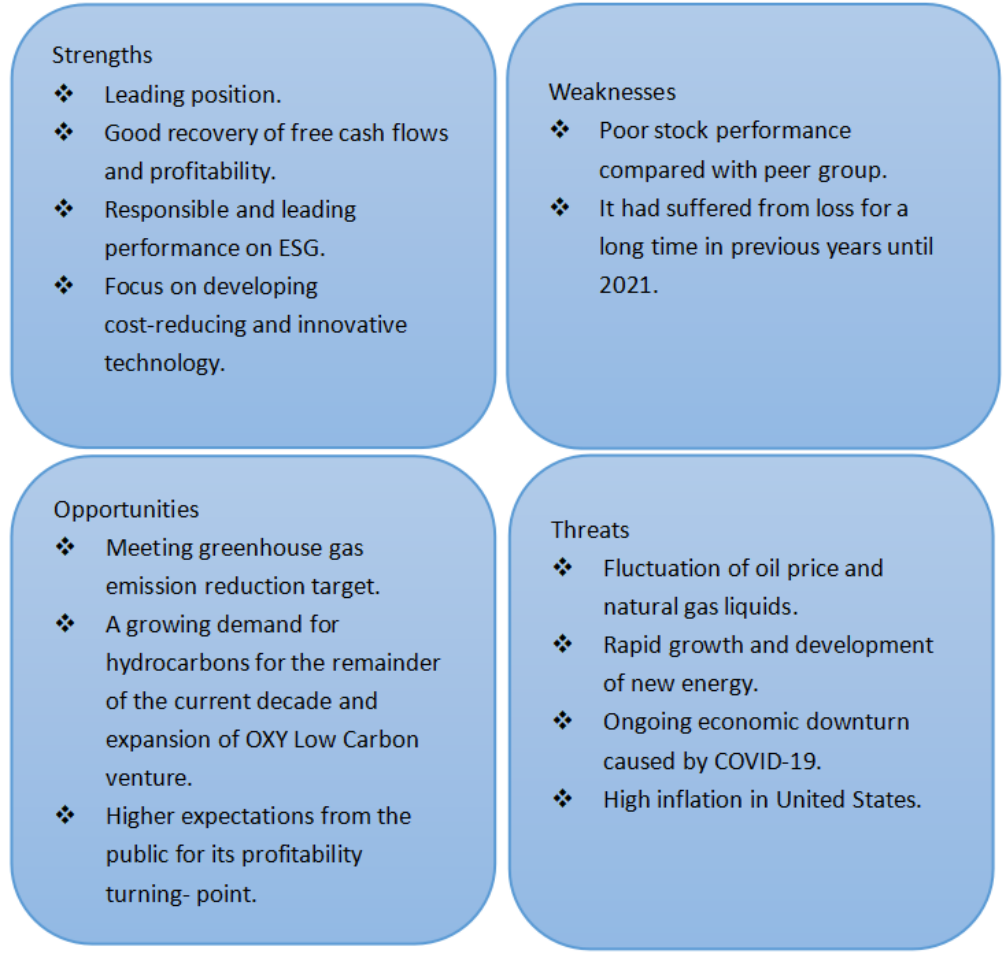
\includegraphics[width=13cm]{Images/SWOT.png}
    \caption{SWOT model}
    \label{SWOT}
\end{figure}
\subsubsection{Strengths}
Oxy is one of the largest oil producers in the U.S., including a leading producer 
in the Permian and DJ basins, and offshore Gulf of Mexico.\par
Responsible and leading performance on ESG, such as sustainability low carbon emission during production. In late 2021, Oxy launched their new Zero In™ brand, which highlights the bold steps they’re taking for a low-carbon future by reducing emissions across our operations and helping others do the same. “Zero In” unites talented workforce’s capacity to advance every part of their business today and strives to lead in carbon management—an extension of their core oil and gas and chemical businesses that can significantly enhance enterprise value.\par
Focus on developing cost-reducing and innovative technology. Throughout 2021, OXY capitalized on efficiency improvements by rapidly deploying new techniques across their operations, enabling them to accelerate time to market for our products while generating meaningful capital savings. OXY achieved record drilling cycle times in the Permian Basin, Rockies, Gulf of Mexico and in Oman, and set new efficiency benchmarks across their portfolio. 
\subsubsection{Weaknesses} 
Poor stock performance compared with peer group\par
The graph compares the yearly percentage change in Occidental’s cumulative total return on its common stock with the cumulative total return of the Standard \& Poors 500 Stock Index (S&P 500), which includes Occidental, with that of Occidental’s peer group over the five-year period ended December 31, 2021. The graph assumes that \$100 was invested at the beginning of the five-year period shown in the graph below in: (i) Occidental common stock, (ii) the stock of the companies in the S&P 500 and (iii) each of the peer group companies’ common stock weighted by their relative market capitalization within the peer group and that all dividends were reinvested. The cumulative total return of the peer group companies’ common stock includes the cumulative total return of Occidental’s common stock.\par
Occidental’s peer group consists of BP p.l.c., Chevron Corporation, ConocoPhillips, EOG Resources, Inc., ExxonMobil Corporation, Shell, TotalEnergies SE (Total) and Occidental.
(Source: annual report 2021 of OXY)
\begin{figure}[h]
    \centering
    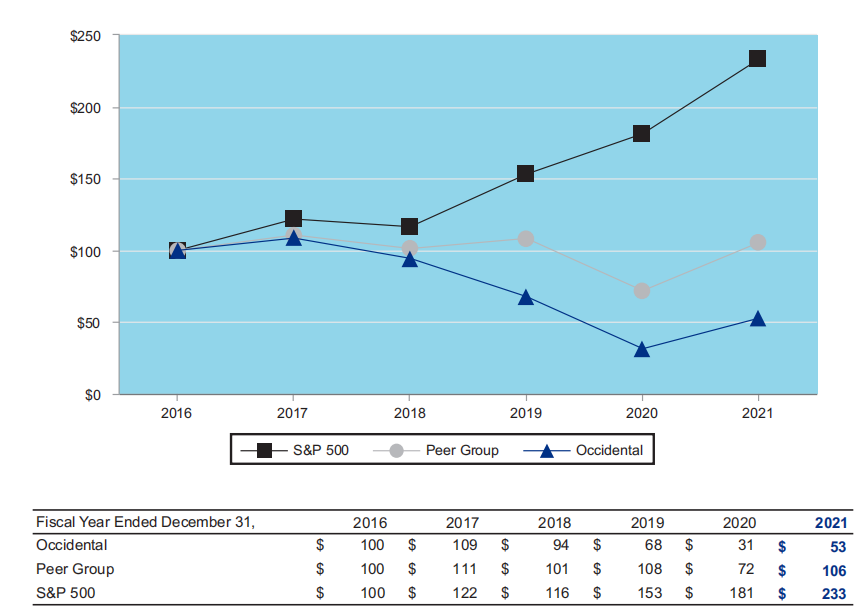
\includegraphics[width=12cm]{Images/Weakness.png}
    \caption{Caption}
    \label{fig:my_label}
\end{figure}
\subsubsection{Opportunities}
Paris Agreement’s 1.5-degree Celsius pathway leads OXY to meet greenhouse gas emission reduction target. The continued implementation of the Paris Agreement is an opportunity for the petroleum industry to transform and upgrade, and for enterprises to demonstrate their social responsibility and innovation capabilities. In December, OXY became the first U.S. upstream oil and gas company to enter into sustainability-linked credit facilities, which include absolute reductions in their CO2 equivalent emissions as the key performance indicator. They set additional short- and medium-term targets for emissions reduction and geologic storage or use of captured CO2. OXY should continue to seize the opportunity to further its influence on ESG while various industry forecasts indicate a growing demand for hydrocarbons for the remainder of the current decade. (Source: annual report 2021 of OXY, Industry outlook)
\subsubsection{Threats} 
Fluctuation of oil price and natural gas liquids influenced by political and economic factors is a threat to OXY. Details can be seen from PESTEL analysis. Rapid growth and development of new energy is also a threat. Details can be seen from Porter’s five forces model analysis.
\subsubsection{SO strategy}
Look for opportunities that make use of strength\par
Strength: Leading position and innovation on ESG performance in crude oil \& natural gas industry.\par
Opportunity: The continued implementation of the Paris Agreement urges the petroleum industry to transform and upgrade\par
Occidental should increase investment on OLCV, Oxy’s low-carbon business and expanded its pursuit of carbon capture projects to realize their net-zero goals and generate significant long-term opportunities. Occidental’s operational flexibility regarding its mix of short-cycle and mid-cycle projects and its knowledge and experience in CO2 separation, transportation, use, recycling and storage means that its oil and gas segment is well positioned to support Occidental’s transition to net zero as well as create opportunities in a low-carbon future.
\subsubsection{ST strategy}
Use strength to overcome or avoid threats\par
\begin{itemize}
    \item \textbf{Strength:} Good recovery of free cash flows and profitability
    \item \textbf{Threat:} Fluctuation of oil price and natural gas liquids
\end{itemize}
These and other factors make it difficult to predict the future direction of oil, natural gas liquids and domestic gas prices reliably. Occidental should continue to focus on allocating capital to its highest-return assets with the flexibility to adjust based on fluctuations in commodity prices. International gas prices are generally fixed under long-term contracts. Occidental should continue to adjust capital expenditures in line with current economic conditions with the goal of keeping returns well above its cost of capital. 
\subsubsection{WO strategy}
Look for opportunities which address weakness\par
\begin{itemize}
    \item \textbf{Weakness:} Poor stock performance compared with peer group.
    \item \textbf{Opportunity:} Higher expectations from the public for its profitability turning- point.
\end{itemize}
Occidental can consider a share repurchase program. Occidental can reward their shareholders with the triple benefit of a sustainable common dividend, a continuously strengthening financial position and an active share repurchase program.
\subsubsection{WT strategy}
Minimize both weaknesses and threats\par
\begin{itemize}
    \item \textbf{Weakness:} Poor stock performance compared with peer group and its being in loss previously.
    \item \textbf{Threat:} Fluctuation of oil price and natural gas liquids and rapid growth of new energy.
\end{itemize}

Occidental should try to diversify risk through preliminary capital investments and long-term contracts to cope with stress brings from both internal weaknesses and external threats.

\section{(李婷婷)Financial Analysis}
To understand the overall operation of a listed company, we can generally consider the four aspects of the enterprise's solvency index (debt ratio, etc.), operating ability index (turnover ratio, etc.), profitability index (profit rate, etc.) and development ability index (growth rate, etc.). However, for Occidental Petroleum Corporation , As the oil industry generally has a large investment scale, long construction and development time, who often encounter the risk of oil price fluctuations in operation will pay more attention to their profitability and solvency. Therefore, we will study and consider  Occidental Petroleum Corporation from the following three aspects: profitability, liquidity and solvency.

\subsection{Profitability}

\subsubsection{ROCE}
First of all, in terms of corporate profitability, ROE (return on equity) is a primary index to measure profitability. ROE refers to the return on equity index, also known as the return on shareholders' equity, which is the percentage formed between the net profit of an enterprise and the average shareholders' equity. ROE is net profit divided by equity. The higher the return on equity is, the more profit the company will make, the higher the income brought by the investment will be, and the development prospect of the company will be clearer. In this ROE study, We selected several representative companies in the oil industry for comparison with Occidental Petroleum Corporation :Exxon Mobil Corporation (XOM), Chevron Corporation (CVX) and Royal Dutch Shell(Shell).

\begin{figure}[h]
    \centering
    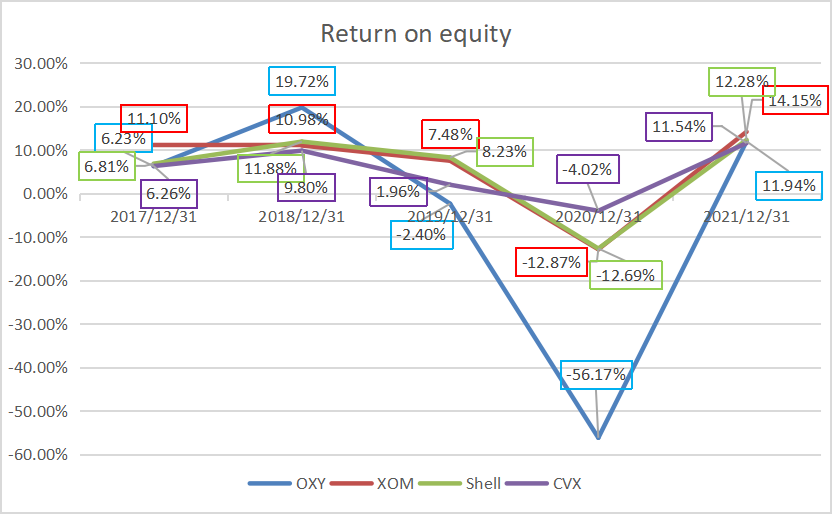
\includegraphics[width=15cm]{Images/return on equity.png}
    \caption{Return on equity}
    P.S. OXY —Occidental Petroleum Corporation ; XOM —Exxon Mobil Corporation; CVX —Chevron Corporation ; Shell —Royal Dutch Shell. The same as in the following tables.
    \label{return on equity}
\end{figure}
\begin{table}[!ht]
    \centering
    \caption{The Liability and Net profit of OXY}
    \begin{tabular}{l|ll}
    \hline
        year & Liability & Net profit  \\ \hline
        2021/12/31 & 54.71 billion & 232.2 billion  \\ 
        2020/12/31 & 61.49 billion & -14.83 billion  \\ 
        2019/12/31 & 72.96 billion & -0.522 billion  \\ 
        2018/12/31 & 22.52 billion & 4.131 billion  \\ \hline
    \end{tabular}
\end{table}
\par
As can be seen from the figure 1, from 2017 to 2021, the ROE index of Occidental Petroleum companies was slightly lower than that of other companies, and maintained a good level only before 2020, but the ROE dropped rapidly after theCOVID-19 pandemic began. We know that the ROE decreases on the one hand because of the increase in liabilities and on the other hand because of the decrease in net profit. According to the financial statements of Occidental Petroleum, in 2018, it was due to the sharp increase in liabilities, such as the amount of liabilities increased from 22.52 billion to 72.96 billion, while the net profit decreased from 4.131 billion to - 0.522 billion, which resulted in the decrease in ROE. In addition, although the debt in 2020 is reduced, the ROE decreases from -2.40\% to -56.17\% due to the sharp decline in net profit. As a result, Occidental's shareholder return indicators are in poor condition.

\subsubsection{Operating profit margin and Asset turnover}
In addition, a deterioration of ROE is either because of low margins or bad use of assets. The decrease may be due to decrease in selling prices or increase in manufacturing (or purchased) costs. They may also be caused by changes in sales mix or inventory counting errors. A change in the operating profit margin is a measure of how well a company has controlled overheads. The asset turnover ratio shows how efficiently the assets are being used. 
\begin{figure}[h]
    \centering
    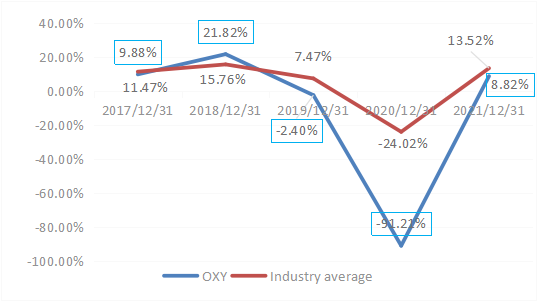
\includegraphics[width=15cm]{Images/The comparison of operating profit margin.png}
    \caption{ The comparison of operating profit margin}
    \label{ The comparison of operating profit margin}
\end{figure}
\begin{figure}[h]
    \centering
    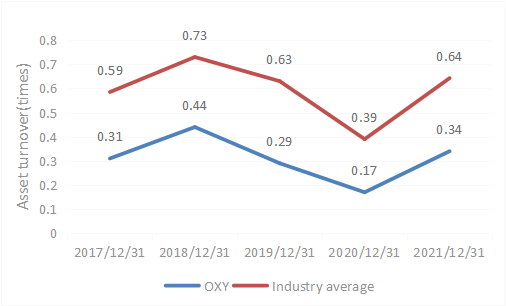
\includegraphics[width=15cm]{Images/The comparison of asset turnover.png}
    \caption{The comparison of asset turnover}
    \label{The comparison of asset turnover}
\end{figure}
\par
From figure 3, we can see that the profit rate of Occidental Petroleum Corporation is generally lower than the average value of the industry. Meanwhile, as shown in figure 4, the total asset turnover rate of  Occidental Petroleum Corporation fluctuates around 0.3 times and is significantly lower than the average value of the industry. However, theoretical studies have found that the asset turnover rate of a company is more appropriate at 0.8 times. Therefore, it can be concluded that the total asset turnover rate of  Occidental Petroleum Corporation is slow and the sales capacity is weak.

\subsubsection{The reasons for low carbon profitability}
In view of the above profitability situation, we summarized the following reasons: 
\begin{itemize}
    \item The drop in oil prices during the COVID-19 pandemic is partly due to a natural drop in oil prices due to low crude consumption. The more important reason is that the three major oil producing countries, in order to compete for customers, have adopted the policy of increasing production and reducing prices to seize the market, which resulted in a substantial increase in production and a decrease in prices. Due to the plunge in oil prices, the company s selling prices have dropped, reducing its net profit.
    \item Due to the influence of the Global Energy Transition program, Occidental Petroleum companies spent too much on research and development of direct air capture technology, which greatly reduced their sales profits. 
    \item The high level of corporate debt, financial expenses, write down the net profit of the enterprise. On the one hand, it is because Occidental petroleum Company acquired Anadarko, which caused it to bear huge debts (more than 30 billion dollars of debts were added to the balance sheet). The reason for this merger and acquisition is that the company can bring Occidental petroleum Company a large area of land in the permian basin rich in oil and gas, which can enable Occidental petroleum Company to maintain its position as the largest oil producer in the permian basin. On the other hand, it may be due to the use of credit sales to expand the market. That's why Occidental's debt levels are so high.
\end{itemize}

\subsection{Liquidity}
To analyze the liquidity of the company is to observe the capital turnover of the enterprise in a certain period of time and master the efficiency of the use of the enterprise capital. Appropriate liquidity indicators can help investors to monitor the company's liquidity situation in time, so as to discover potential risks and respond to them in time.
 In this study, we mainly used current ratio and quick ratio to analyze.
 \begin{figure}[h]
     \centering
     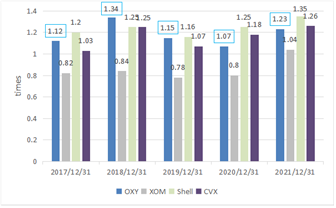
\includegraphics[width=15cm]{Images/comparison of current ratios.png}
     \caption{The comparison of current ratios}
     \label{The comparsion of current ratios}
 \end{figure}

\begin{figure}[h]
    \centering
    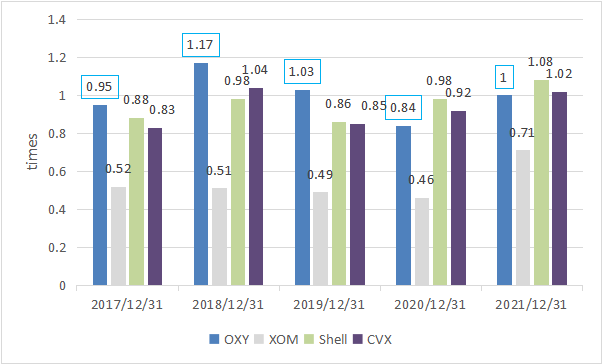
\includegraphics[width=15cm]{Images/Comparison of quick ratio.png}
    \caption{Comparison of quick ratio}
    \label{comparison of quick ratio}
\end{figure}
 
These ratio measures the ability of the company's current assets to immediately pay off its current liabilities. 
Current ratio reveals the guarantee degree of current assets to current liabilities, examines the security of short-term debt repayment, and represents the realization ability of enterprises. The quick ratio is used to measure the ability of an enterprise's current assets to immediately pay off the maturing debt. Compared with the current ratio, quick ratio can more accurately and reliably evaluate the liquidity of enterprise assets and its ability to repay short-term liabilities because it excludes the assets with weak and unstable liquidity such as inventory.  From figure 5, we can see that Occidental's current ratio, which was slightly higher than that of several other oil companies in 2018, is generally slightly lower than that of several other oil companies in 2017-2021, maintaining a level of 1.1 times. This is a bit different from the standard current ratio of 1.5-2.0 times that is widely accepted in the industry.  As can be seen from figure 6, the quick ratio of occidental oil companies is also maintained at the level of 0.9 times, which is a normal situation. We know that the current ratio is generally better between 1.5 and 2.0, and the quick ratio is better around 1.0. However, as can be seen from figure 5 and 6, compared with other companies, Occidental Petroleum has general liquidity, low liquidity ratio and quick ratio, and low capital utilization efficiency, such as inventory overhang, cash surplus and other problems, so its short-term solvency is weak. 
\par
Here's why Occidental's liquidity is lower than the industry average: 1. Backlog. Due to the impact of the epidemic, the price of oil plummeted and the demand for oil declined, leading to a decline in sales, and some goods could not be sold, resulting in a backlog in the warehouse. 2. Enterprise monetary funds idle. 3. Too much receivables.

\subsection{Solvency}
\begin{figure}
    \centering
    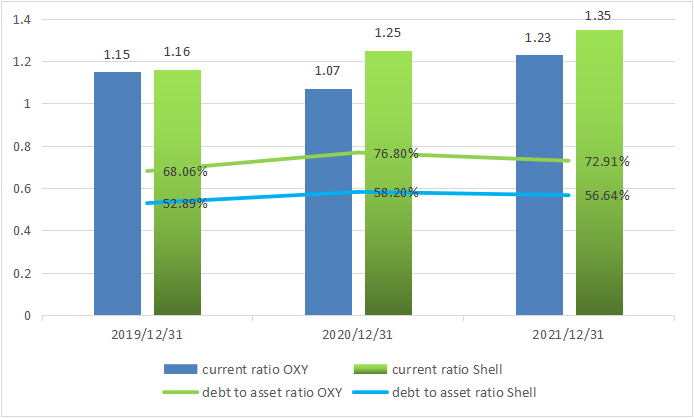
\includegraphics{Images/The current ratio and debt to asset ratio between OXY and Shell.png}
    \caption{The current ratio and debt to asset ratio between OXY and Shell}
    \label{The current ratio and debt to asset ratio between OXY and Shell}
\end{figure}
Solvency reflects whether an enterprise has the ability to repay debts in time according to the agreement. Whether an enterprise has the ability to pay cash and repay debt is the key to its healthy survival and development. The solvency of an enterprise is an important symbol that reflects the financial condition and operating ability of an enterprise. Debt to asset ratio is the percentage of total liabilities divided by total assets, that is, the ratio of total liabilities to total assets. The debt to asset ratio reflects how much of the total assets are financed by borrowing, and can also measure the extent to which an enterprise protects the interests of creditors in liquidation.
\par
Aiming at the solvency of enterprises, we compare the relationship between the debt to asset ratio and current ratio of Occidental Petroleum and Shell. As can be seen from the figure 7, compared with Shell Company, Occidental Petroleum Company's debt to asset ratio is higher than Shell company's, but its quick liquidity ratio is lower. Occidental Petroleum Company undertakes large debts, but its short-term repayment ability is low, so the enterprise financial risk is high. 
\par
Although the debt paying ability of enterprises is relatively weak, that is, the financial risk of enterprises will be high when the debt ratio is high and the liquidity ratio is low, it also has some advantages: for the high debt ratio of enterprises, the leverage of enterprises is high. Through leverage, enterprises can enlarge the operating earnings, and enterprises can exchange more debt (that is, shareholders themselves invest less capital) for higher returns. The risks are also obvious. Debts usually require fixed interest payments. If the enterprise cannot generate enough profits and cash flow to cover the financial costs, the enterprise will collapse.
\par

\subsection{4.4 The advice about the operation of OXY}
Finally. We have the following suggestions on the profitability, liquidity and solvency of an enterprise: 
\begin{enumerate}
    \item low profitability
    \begin{enumerate}
        \item Reduce the finance expense of interest on debt. The most important method is to properly adjust and reduce the expansion speed of enterprises and reduce the generation of debt;
        \item Strengthen the management of current assets and reduce the period expenses which can reduce the cost of profit write-down impact, improve the profit margin;
        \item Adopt the way of small profits and quick sales to accelerate the turnover of assets and increase sales. 
        \item Category expansion is an effective way to reduce the impact of oil price fluctuations. Some high-value petroleum products will increase the overall profits of the company, and different petroleum products have different responses to oil prices, which can effectively reduce the uncertainty caused by large changes in oil prices and thus improve the profitability of enterprises.
        \item Have a reasonable planning of production schedule. In the whole petrochemical industry chain, from upstream oil exploitation to downstream sales of finished products, the profitability of each link has different sensitivity fluctuations to oil prices. For example, when oil prices rise, upstream oil exploration and production, refining business will improve profitability, at this time the company should increase upstream oil storage and production, improve refining production plan to achieve profitability.
    \end{enumerate}
    \item Bad rapid solvency and Low capital utilization efficiency—Increase sales and reduce inventory overhang which can improve asset turnover speed;The comprehensive management of fixed assets is an important way to improve the utilization rate of assets. Reducing the idle assets, artificial loss of equipment and loss of assets can extend the service life of assets, speed up the turnover of assets and reduce the occupation of funds, so as to reasonably reflect the value of assets and truly reflect the production and operation conditions of enterprises.
    \item 3.	High financial risk—Have a scientific debt and optimize the capital structure, in order to reduce financial risk. Therefore, the enterprise must carry out reasonable planning. According to the amount of borrowing, the duration, urgency, structural characteristics, and the level of affordable interest rates, the advantages and disadvantages of various debt raising methods should be combined with their own actual needs, affordability, possible future income, and the degree of risk impact on their own asset structure to carefully select the most suitable and least risky financing method, In this way, the risk of insolvency can be reduced to the lowest point. We can adjust corporate capital structure, return long-term debt in advance, and convert part of debt capital into equity capital.
\end{enumerate}

\section{(叶炯尧)Corporate-level Analysis}

\subsection{Mission and Goals}
\subsubsection{Zero In}
Occidental Petroleum is taking a number of steps to innovate for a low carbon future. They are exploring new ways to reduce emissions in their energy and chemical businesses, while providing products and services to help others do the same, with the goal of achieving net zero emissions.
\subsubsection{Producing vital energy to sustain people and our planet}
Occidental Petroleum continuously enhance its operations to deliver the energy that lifts up societies and economies around the world, while innovating new approaches to advance global sustainability.
\subsubsection{Essential chemistry for indispensable purposes}
In its legacy of more than 100 years of leadership, OxyChem has achieved progress toward a safer world with a higher standard of living. They are a first-class producer nationally and globally for all the chemicals they produce and sell, with a reputation for prioritizing safety, environmental protection, customer service and sustainability to be the Partner of Choice.
\subsubsection{Advancing a low-carbon future}
"Together we can take on greenhouse gas emissions". True progress in the fight against climate change means cooperation. That’s why Occidental Petroleum offers powerful, practical solutions other industries can use to decarbonize—including developing net-zero oil and fuels, geologic CO2 storage and carbon management advisory services.

\subsection{BCG matrix}
The BCG matrix, also known as a growth/share matrix, is a strategic management tool that was created by the Boston Consulting Group, which helps in analyzing the position of a strategic business unit and the potential it has to offer. The matrix consists of 4 dimensions, each of which represents a particular product or business, with a vertical axis that represents growth and a horizontal axis that represents market share.
\begin{figure}[H]
    \centering
    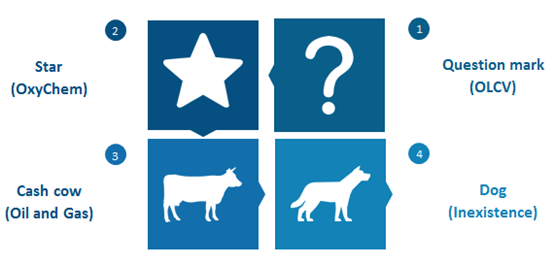
\includegraphics[width = 10cm]{Images/BCG matrix yjy.png}
    \caption{BCG matrix for Occidental Petroleum}
    \label{BCG_matrix}
\end{figure}
\subsubsection{Question mark-“Low Carbon Ventures”}
The “Low Carbon Ventures” is a question mark for Occidental Petroleum. Vicki Hollub, Occidental's chief executive, once said: "Within 15 to 20 years, the company's revenues from carbon management will exceed those from oil and gas." The figure \ref{Historic_emmission} shows that United States is focusing more towards low carbon. Therefore, this market has a high market growth rate. OLCV was established to execute Occidental's vision of reducing global emissions and providing a more sustainable future by developing low-carbon energy sources and products. 
\begin{figure}[h]
    \centering
    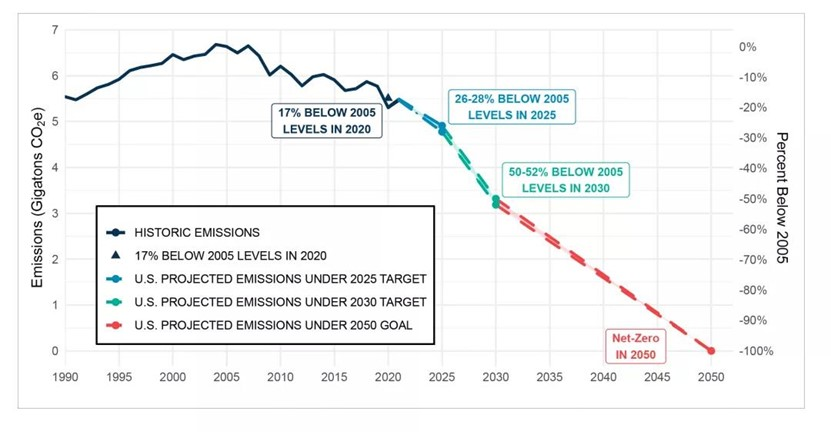
\includegraphics{Images/US historic emissions and projected emissions under the 2050 goal for net-zero.jpg}
    \caption{US historic emissions and projected emissions under the 2050 goal for net-zero}
    Source: The Long-Term Strategy of the United States
    \label{Historic_emmission}
\end{figure}
\begin{figure}[H]
    \centering
    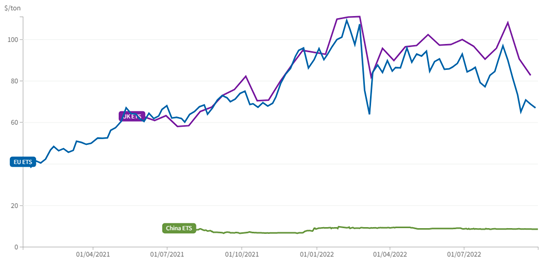
\includegraphics{Images/carbon market price trend.png}
    \caption{Carbon market price trend}
    Source: \url{https://icapcarbonaction.com/en/ets-prices}
    \label{CarbonMarketPrice}
\end{figure}
Under the "net zero" target, Occidental continuously explores the development of carbon capture and storage (CCS) business to reduce carbon emissions. What's more, "Low Carbon Venture" company researches and develops direct air capture (DAC) technology. The technology is already being used in the "net zero" deal that was concluded in early 2022. There is no doubt that Oxy sees great potential for DAC technology applications, and the growing market for carbon credits and low carbon fuels will accelerate the commercialization of DAC technology.

However, Oxy has a low market share in this segment because OLCV is just a new business. \par
OLCV, in partnership with Macquarie Group and Global Markets Group, has delivered 2 million barrels of carbon-neutral oil to India's Reliance Industries in 2021, according to overseas media reports on Jan. 29. \par 
Since OLCV is advancing leading-edge technologies and business solutions that economically grow our business while reducing emissions, the recommended strategy for Oxy is to invest in research and development to come up with innovative features. That may mean forgoing short-term gains in favor of long-term development.

\subsubsection{Star-OxyChem}
OxyChem is a leading producer of life enhancing chemistry with facilities in the United States, Canada and Latin America. It primarily manufactures and markets basic chemicals and vinyls. As a market leader, OxyChem's market position was first or second in the U.S. for the principal chemistry. Besides, OxyChem ranks in the top three producers of PVC in the United States.
\par
Table \ref{PrincipleProducts} shows the principle products of OxyChem.

\begin{table}[!ht]\footnotesize
    \centering
    \caption{Principle Products}
    \label{PrincipleProducts}
    \begin{tabular}{lll}
    \hline
        Principal Products & Major Uses & Annual capacity  \\ \hline
        \textit{\textbf{\color{Blue}Basic Chomicals}} & ~ &   \\ 
        chlorine & Raw material for ethylene dichloride (EDC) water \\ & treatment andpharmaceuticals & 3.2 million tons  \\ 
        Caustic soda & Pulp paper and aluminum production & 3.3 million tons  \\ 
        Chlorinated organics & Refrigernis) silicones and pharmaccuticals & 1.0 billlon pounds  \\ 
        Potasslum chemicals & Fertilizers, batteries, soaps, detergents and specialty glass & 0.4 milllon tons  \\ 
        EDC & Raw material for VCM & 21 billion pounds  \\ 
        Chlorinated isocyanurates & Swimming pool sanitation and disintecting products & 131 million pounds  \\ 
        Sodium silicates & Catalysts, soaps, detergents and paint pigments & 0.6 million tons  \\ 
        Calcium chloride & lce melting. dust control, road stabilization and oil field services & 0.7 million tons  \\ 
        \textit{\textbf{\color{blue}Vinyis}} & ~ &   \\ 
        VCM & Precursor for pyc & 6.2 billion pounds  \\ 
        PVC & Piping, building materials and automotive and medical products & 3.7 billion pounds  \\ 
        Ethylene & Raw material for VCM & 1 .3 billion poundsei  \\ \hline
    \end{tabular}
\end{table}
According to relevant information, the overall category is expected to grow at high market growth rate in future. Figure \ref{PVC} presents the global PVC production from 2016 to 2020. In 2021, the United States economic growth, estimated to be 5.6\%, was significantly higher than the 3.4\% contraction experienced in 2020, which resulted in higher demand for most products including caustic soda and PVC. Prices for PVC continued to remain strong in 2021 due to increased domestic demand and record high pricing in global markets. Demand for basic chemicals in 2022 is expected to improve further from 2021 levels.
\begin{figure}
    \centering
    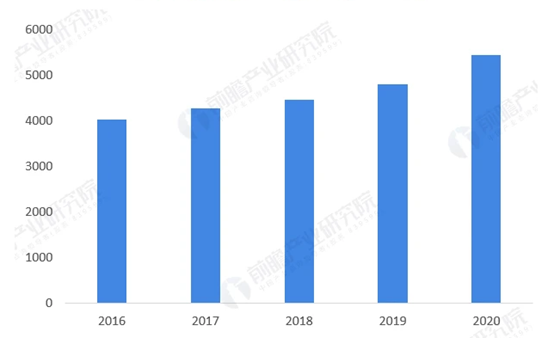
\includegraphics{Images/Global PVC Production from 2016 to 2020.png}
    \caption{Global PVC production, 2016-2020 (unit: 10,000 tons)}
    Source:\url{https://bg.qianzhan.com/trends/detail/506/220711-bf3062e7.html}
    \label{PVC}
\end{figure}
Therefore, OxyChem is a star and should use its current products to penetrate the market. It's of great importance to main the current situation as longer as it can. This could be done by improving its distributions that will help in reaching out to untapped areas. In addition, Oxy's low-carbon division used man-made carbon dioxide (CO2) instead of hydrocarbon feedstock to produce ethylene. Ethylene is widely used in the chemical industry as a component of products ranging from plastic film to polyvinyl chloride pipes and coolants. The new technology uses carbon dioxide, water and light to produce ethylene, helping to reduce costs and carbon emissions.
\subsubsection{Cash cow——Oil and Gas}
Occidental’s oil and gas assets are characterized by an advantaged mix of short-cycle and long-cycle high-return development opportunities. This has been in operation for over decades and has earned Oxy a significant amount in revenue. Oxy primarily conducts its ongoing exploration and production activities in the United States, the Middle East and North Africa. \par
With the completion of the Acquisition, Oxy became one of the largest U.S. producers of liquids, which includes oil and NGL. 
\begin{figure}[H]
    \centering
    \caption{Comparative oil and gas proved reserves and sales volumes}
    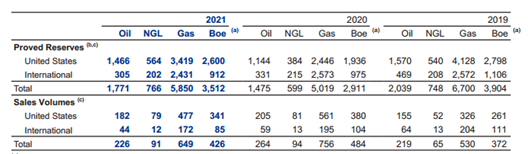
\includegraphics{Images/Comparative oil and gas proved reserves and sales volumes.png}
    Source: \url{https://www.oxy.com}
    
    \label{Comparative oil and gas proved reserves and sales volumes}
\end{figure}
\begin{figure}[H]
    \centering
    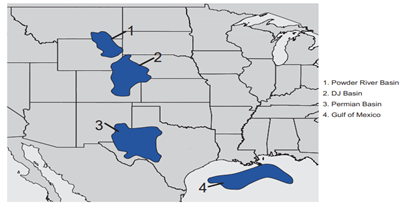
\includegraphics{Images/domestic assets.png}
    \caption{Domestic assets}
    Source: \url{https://www.oxy.com}
    \label{Domestic assets}
\end{figure}
\begin{figure}[H]
    \centering
    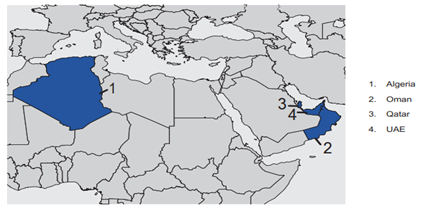
\includegraphics{Images/Oversea assets.png}
    \caption{Oversea Assets}
    \label{Oversea Assets}
\end{figure}
As a producer of oil, NGL and natural gas, Occidental competes with a competitive environment. Oil, NGL and natural gas are sensitive to prevailing global and local market conditions, as well as anticipated market conditions. In the future, oil prices will continue to be affected by global supply and demand, which are generally a function of global economic conditions, inventory levels, production or supply chain disruptions, technological advances, regional market conditions and the actions of OPEC, other significant producers and governments. Moreover, transportation capacity, currency exchange rates and the effect of changes in these variables on market perceptions, these are all factors to consider.
\begin{figure}[h]
    \centering
    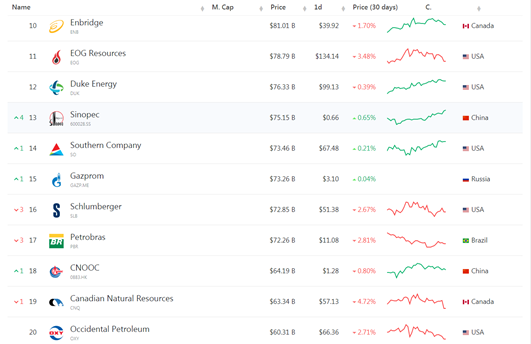
\includegraphics{Images/Oil and gas companies market cap.png}
    \caption{Oil and gas companies market cap}
    Source: \url{https://companiesmarketcap.com/oil-gas/largest-oil-and-gas-companies-by-market-cap}
    \label{Oil and gas companies market cap}
   
\end{figure}
Besides, the future of clean energy investment is much bigger. As mentioned above, companies' revenues from carbon management will exceed those from oil and gas within 15 to 20 years. This change in trends has led to a decline in the growth rate of the market.
\par
After all, oil and gas forms an important part of the company and should be retained and maintained. There is also the fact that the success of the shale gas and oil revolution
in the United States has resulted in the United States being the only country in the world to commercially exploit shale oil and gas resources. Currently, Occidental’s competitive strategy relies on maintaining production in a capital efficient manner. Such as developing conventional and unconventional fields and utilizing primary and enhanced oil recovery (EOR) techniques. Oxy can focus on cost-reduction efficiencies and innovative technologies to reduce carbon emissions in the future.
\subsubsection{Dog——Inexistence}
A dog is a product or business unit with a low market share and in a low-growth market. Dog can tie up funds and provide a poor return. In general, they should be sold off although 	may be retained if they are a useful niche business. However, no business lines or subsidiaries meeting this definition can be found on Occidental's official website or related information. In October 2021, the OXY completed the sale of its Ghanaian assets. Prior to the divestment, the Ghana operations included offshore production and development activities. Occidental’s net share of production in 2021 was 16 Mboe/d. But it was obviously a business that had to be abandoned to pay off a debt, not a dog.
\subsection{Ansoff matrix}
Ansoff Matrix takes product and market as two basic aspects, and distinguishes four product/market combinations and corresponding marketing strategies. It is one of the most widely used marketing analysis tools. Its main logic is that an enterprise can choose four different growth strategies to achieve the goal of increasing revenue.
\begin{figure}[H]
    \centering
    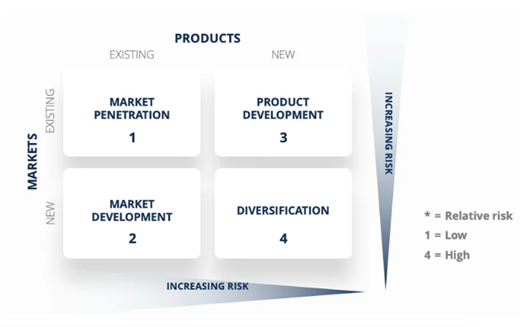
\includegraphics{Images/Ansoff Matrix.png}
    \caption{Ansof Matrix}
    Source:\url{https://corporatefinanceinstitute.com/resources/management/ansoff-matrix/}
    \label{Ansof Matrix}
    
\end{figure}
\subsubsection{Market Penetration}
Market penetration means increasing market share of existing products. It’s a low-risk strategy since it requires no capital investment. Occidental Petroleum has the advantage of ultra-low production costs. The Permian Basin is believed to be one of the largest known oil reserves in the United States and one of the cheapest places in the world to drill for oil. The acquisition of Anadarko three years ago boosted Occidental's holdings in the U.S. Permian to 2.8 million acres. That makes Oxy one of the Permian's biggest producers and one of the cheapest, with production costs of just \$40 a barrel.
\par
Lower production costs mean that Oxy has a higher margin of safety and a wider margin of profit in the face of volatile oil prices. The price of WTI crude oil is still high at \$88 per barrel, even though the international oil price is lower than in recent months. Oxy can use lower prices to attract more potential customers and thus achieve market penetration.
\subsubsection{Market Development}
Market development means seeking new customers for existing products. The risk is still reasonably low.
% \begin{figure}[H]
%     \centering
%     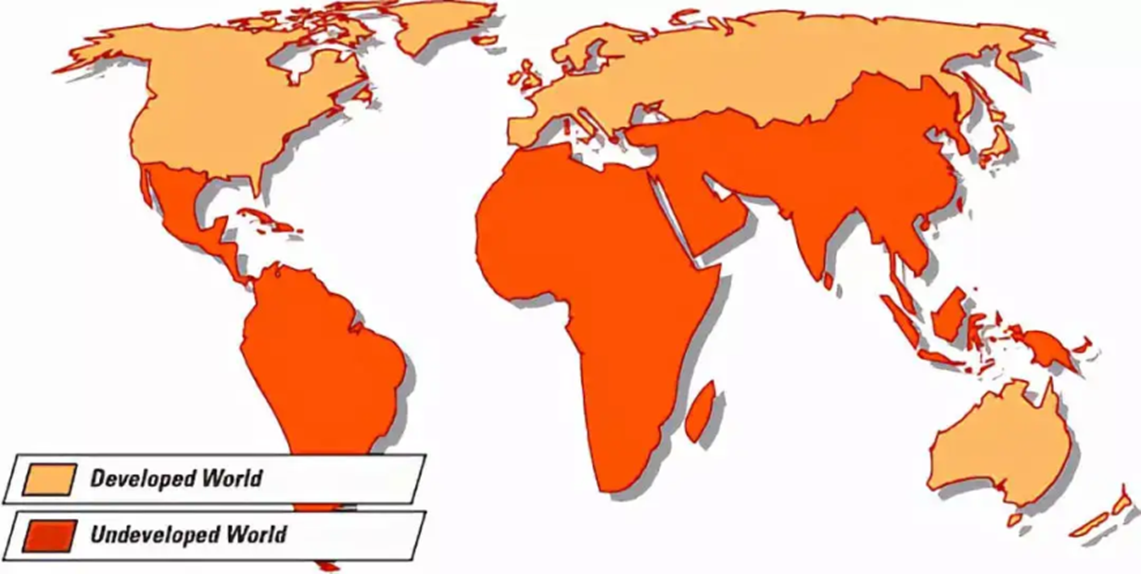
\includegraphics{Images/developing countries.png}
%     \caption{Developed and developing countries}
%     \label{Developed world}
% \end{figure}
Oil demand is not likely to peak any time soon because of the greater development needs of developing countries. The emerging middle classes in developing countries can be expected to aspire to travel in ways similar to those in developed countries. The new wealth is also driving demand for consumer goods made from or packaged in plastic, which is made from oil and natural gas. So Oxy can try to tap into developing countries to achieve market development.
\subsubsection{Product development}
Product development means selling new products to existing customers. This strategy is riskier than both above since it is likely to require major investment in R&D process and production facilities.\par
Enhanced Oil Recovery (EOR) refers to the injection of carbon dioxide into producing fields to help improve the operational, financial and environmental performance of the reservoir. Hydrocarbon producing rocks are porous. The injected carbon dioxide displaces the oil and gas trapped in the porous rock, and then partly traps itself. This technique traps CO2 permanently in the reservoir while producing oil more efficiently. Continued use of EOR technology for product development can improve Oxy’s operational efficiency and achieve the goal of Net-Zero Oil. It can also increase sales revenue from existing customers. 
\subsubsection{Diversification}
Diversification means selling new products to new customers, it may offer significant growth potential but it is risky as it may require significant investment and new competences. Occidental Petroleum has invested huge sums in building carbon capture and carbon removal plants. It set up a company called 1PonitFive in 2020, symbolizing the Paris Agreement's maximum goal of keeping global warming below 1.5 degrees Celsius.
\par
With the diversification, Oxy have come back from the dead. In 2020, the company posted a full-year loss of \$14.8 billion. In the first half of 2022, the company posted a net profit of \$8.6 billion.
Figure \ref{Global budget} shows the line graph of changes of global Fossil Carbon-dioxide emissions.
\begin{figure}[H]
    \centering
    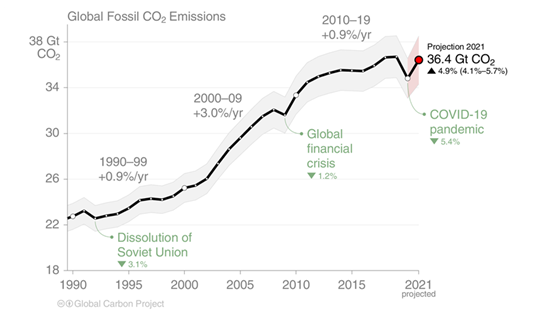
\includegraphics{Images/Global Budget.png}
    \caption{Global budget}
    \label{Global budget}
\end{figure}
Source: https://doi.org/10.18160/gcp-2021
\subsubsection{Sell carbon credits}
Companies need to offset carbon emissions because they have a net zero target. According to the Net Zero Tracker, nearly 40\% of the world's largest 2,000 publicly traded companies have a net zero target. Airbus, the maker of the world's superjumbo aircraft, has pre-purchased carbon credits from Oxy.
\subsubsection{Sell zero-carbon crude oil}
Oil drillers used to pump carbon dioxide into Wells to enhance oil recovery, and Oxy was the leader. In the future, it will use the carbon it captures to do the technology. Most importantly, Oxy can even turn zero-carbon oil into "negative carbon oil”. Oxy see carbon not as waste, but as something that adds value to a product.

\subsection{Four Scenario Analysis}
Although the dramatic shift in the energy landscape is old news, many of the factors affecting it are still changing rapidly. Therefore, we divide Occidental's future development into four scenarios by analyzing the consumer, technology, and government orientation.
\subsubsection{Meet in “Paris”}
The first scenario depicts the most optimistic hypotheses of a transition to low or no carbon energy. With rapid technological advances, alternative energy sources will soon be able to replace existing conventional energy sources at a lower cost. On the one hand, consumers' awareness of environmental protection is constantly improving, and their lifestyles have undergone great changes. On the other hand, countries agree to limit and ban carbon trading for internal combustion engines, which is in line with the goals of the Paris Agreement. So we recommended OXY adopt the strategy of developing new energy sources, such as electric vehicle charging and renewable fuels.
\subsubsection{“The Long Goodbye”}
Renewable energy market share grows in the "long goodbye" scenario. Although oil demand has peaked, inventory effects, consumption inertia and the continued growth of the aviation and petrochemical industries have prevented a significant decline in oil demand. In this scenario, we assume that the cost and performance improvements of new energy products are not sufficient to persuade consumers to quickly abandon their existing assets. Although the government will continue to support the energy transition, there will be some obstacles in the process. National policies to mitigate climate change have gradually increased, but budget pressures and global political uncertainty have prevented the goals of the Paris Agreement from being fully achieved.\par
We believe that technological developments will not stand still, and with continued government support for the energy transition, it is only a matter of time before consumers become familiar with and adapt to new technologies. With these factors coming together, Oxy should adopt a digital strategy, using computer technology to collect more data, perform more sophisticated analysis and establish more precise process controls to reduce the cost.
\subsubsection{"Snail"}
As mentioned above, Oil demand is not likely to peak in the developing countries. While the cost of alternative energy sources is falling, the oil and gas industry is also digitizing, and the cost of finding, extracting, and transporting oil and gas resources is falling. The dominance of renewable energy over hydrocarbons has been slow. In addition, since the cost advantages of alternative energy sources are not outstanding, the government is paying less attention to climate change and other environmental issues. Even if electric vehicles are competitive in terms of cost and performance, it will take time for consumers to recognise their advantages. 

\subsubsection{Key natural gas}
In the final scenario, as consumers move towards electric vehicles, oil demand peaks and soon declines. Renewable technologies have cost advantages, but capital markets cannot immediately transfer the capital needed from companies to consumers. The lack of capacity in coal-fired or nuclear power plants needs to be filled in other ways, making natural gas a competitor or complement to renewables. The complementary relationship between gas and renewables will be skewed towards gas. In the near and medium term, if all the new electricity comes from renewable energy, the operating cost of the power system is likely to be very high. Besides, consumers can't or won't pay for distributed solar on a large scale. Occidental Petroleum has therefore adopted a strategy of further developing its gas-related assets (including upstream, midstream and downstream).

\subsubsection{Section Summary}
Frist, Oil demand may be peaking in the future. Battery technology is already advanced and will continue to improve, making electric vehicles cost and performance competitive with internal combustion engines. Like any commodity enterprise, the biggest financial risk of Oxy is the risk of price fluctuation. Supply could outstrip demand, prices could collapse and profits could evaporate. But over time, supply and demand will come into balance. Our response relies on digital technology, continuing to reduce the cost of all processes, and actively expanding into developing markets.
\par
Second, natural gas has a chance to be a market mover. Broken down, the future of oil and gas is not the same. For oil, uncertainty reigns supreme. Oxy can leverage their unique position in the capital markets to drive upstream gas growth by facilitating investment in new downstream branches of the gas industry.
\par
Finally, in the short term, returns from oil and gas projects are likely to remain competitive. The core business lines of the oil and gas industry will remain a core part of the future energy mix. But there are many possible outcomes, and some companies will hedge their investment risk by buying, developing and nurturing other options. Occidental Petroleum should invest in the power sector, charging electric vehicles and renewable fuels as fast as they can.

\section{(许庭悦)Business-level strategy}
Occidental Petroleum Company is a multinational Company with great recognition in its target market segments. However, the intensifying competition has made it challenging for Occidental Petroleum Company to sustain as well as increase the market share without exerting significant efforts. Oxy (Occidental Petroleum) Company has to gain a key strength in its business level in order to maintain its market position and further boost profitability in nowadays economic environment. As a global brand with a strong global power, Occidental has positioned itself on the basis of a number of key factors that give it a strong advantage over its competitors (including competitors) in most consumer markets. Occidental Petroleum Corporation's business level strategy can be understood according to Michael Porter's general model. \par
Michael Porter’s generic strategies, was proposed by Michael Porter in 1980. This model describes how an enterprise pursues competitive advantage by choosing the right strategy. Three main strategies are put emphasis on in the model- Cost leadership Differentiation and Focus. Companies can use competitive advantages by reducing costs or differentiating their products from competitors in the most valuable ways to justify a premium. Companies can also gain a competitive advantage by choosing a narrow focus strategy through niche marketing, a wide focus strategy (by offering products to selected market segments), or an industry-wide strategy (by offering products to the largest market segments) Porter thought that all the companies would only choose on strategy in this generic model, because implementing any strategy effectively usually requires an all-out effort and an organization that supports the strategy. If the enterprise has more than one fundamental goal, the resources in these areas will be dispersed. However, in today's globalized days, it is difficult to choose only one strategy as a business level strategy to stand firm in the market. Because sometimes companies will pursue more than one basic goal, multiple strategies can make a company more dynamic and spread risk.
\par
Occidental Petroleum Company has adopted the strategy of Cost leadership Differentiation and Focus strategies to cope with competitive pressure and achieve the growth objectives.
\subsection{Cost leadership}
Cost leadership strategy is a strategy for enterprises to reduce costs through effective ways, so that the total cost of enterprises is lower than the cost of competitors, or even the lowest cost in the industry, so as to obtain competitive advantages. As for Occidental, it highlights cost leadership as the main strategy to preserve market position through efficient value chain management.
\par
In order to better reflect OXY's cost volume across the oil industry, we compared the cost of sales of oxy with other four leading oil companies from 2009 to 2021, including Exxon Mobil Company, ConocoPhillips Company, Chevron Corporation and Royal Dutch Shell Company. Figure \ref{COGS} shwos the line graph of cost of sales of the above oil companies in the past 2 decades.
\par
\begin{figure}[h]
    \centering
    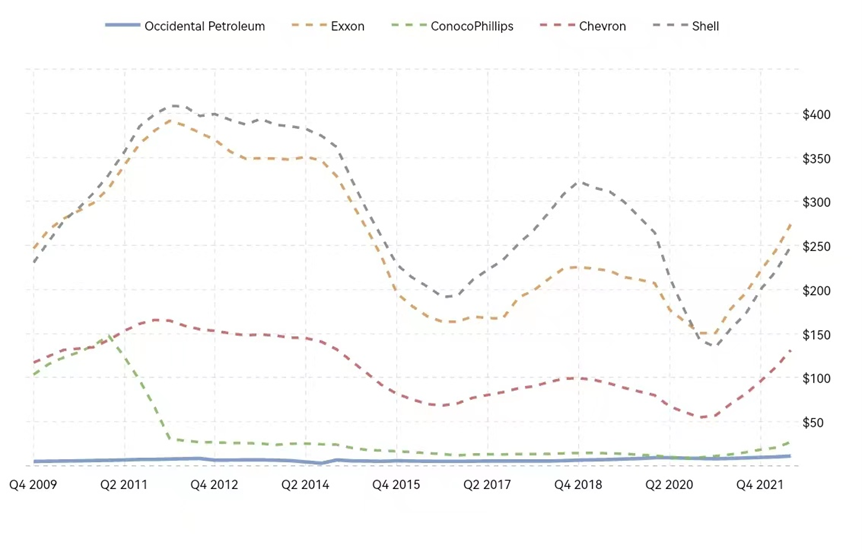
\includegraphics{Images/COGS.png}
    \caption{The cost of sales comparison}
    \label{COGS}
\end{figure}
 According to the data, it's easy to find that the cost of oxyhas always been at the lowest level, which is around \$40 per barrel in average. And for its U.S. operations in 2022 according to OXY’s official website, the company's production costs are less than\$10 a barrel even at low commodity prices, which is significantly below the domestic average.
 \par
In our opinion, there are 3 main strong points to keep a low cost for Occidental——oil field location, production technique and sales \& supply.
\begin{enumerate}
    \item Occidental prefers projects in more mature or ignored oil fields instead of big-ticket drilling projects
    \par
    The main products of oil companies are oil and natural gas, and the cost of oil extraction is affected by the difficulty and quality of the oil field itself, in addition to the extraction technology. As a result, mature fields can boost production and also reduce the exploitation cost. For example, it is the largest producer in the Permian Basin, which is a heavily exploited oil field in Texas and New Mexico. Compared with other oil companies, Occidental Petroleum was founded in 1920, which was late compared with other companies in the oil industry. Due to this, it failed to seize the initial market share. Therefore, as a new competitor who wanted to enter the oil market, it was a wise choice to start their business and completed its first commercial oil well in Permian Basin, because big-ticket drilling projects truly takes a long time and requires huge start-up capital ,which is not conducive to the rapid growth of a new company.
    \item Occidental has been paying attention on new technology to lower the cost. \par
    Improving economic efficiency through exploitation technology innovation has always been a very important way to reduce costs in the oil industry. For most American oil company, the native shale oil is difficult to extract, With the development of technology in the United States, Occidental Petroleum pioneered advanced fracking techniques in the 1990s. As mentioned in the paper, Occidental is the largest producer in the Permian, where it is using enhanced oil-recovery techniques, such as C02 flooding, to extract hard-to-reach oil from the field, which expanded the oil yield of extraction.
    \begin{figure}[h]
        \centering
        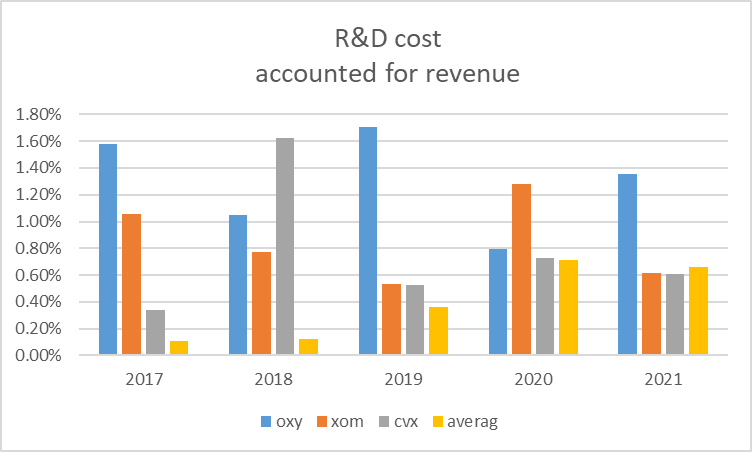
\includegraphics{Images/rd cost.png}
        \caption{The R&D cost accounted for revenue}
        \label{rd cost}
    \end{figure}
    Additionally, instead of being satisfied with traditional fracturing technologies, OXY has been improving and developing new technologies. In the past five years, the company has invested more research and development expenses than the average level of the industry and industry leaders, which is beneficial to improving the production efficiency of enterprises and reducing costs in the long run.
    \item Occidental has a streamlined and efficient sales and supply chain and procurement system
    In today's rapidly developing society, the use of high and new technology to reduce costs is not only in the actual production link, in the sales and transportation link of high efficiency is vital importance. In today's rapidly developing society, the use of high and new technology to reduce costs is not only in the actual production link, in the sales and transportation link of high efficiency is also crucial. Based on OXY’s official website, it shows that the company chooses dedicated, knowledgeable professionals on each account and ensures that they truly understand customers specific needs to reduce communication costs. OXY also uses online order and payment system and b2b Supply Chain Integration service, which digitizes production plans, purchase orders, sales orders, order confirmations, shipping notices, invoices and payments to virtually eliminate manual paperwork. Paperless management in supply and sales link help sell more oil and gas products in a period, thus gaining more profits and expanding economic benefits and improving the company's entire value chain to eliminate or avoid activities that cost money, which truly saves the time cost.
\end{enumerate}
\subsection{Differentiation}
Differentiation strategy is to provide differentiated products or service to form uniqueness in the whole industry. Occidental Petroleum uses differentiation strategy in its market targets and industrial transformation to achieve growth objectives.
\begin{enumerate}
    \item  Occidental expands the market share by targeting the mid end customer market.\par
    To get a better idea of Occidental's customer target market, we looked online for the company's 2021 customer list. Out of a list of 320 major customers we could find, 91.2\% percent of Occidental's customers are medium-sized enterprises (revenue in 2021 under \$20000 million ), which makes the largest proportion of overall consumer market mix in most of the countries. This kind of customers generally place high importance to the pricing factor, although a single purchase of oil is small, the volume can make up for it. The low-cost strategy of Occidental Petroleum not only ensures its profit return but also caters the needs of this consumer segment, differentiated oil products in the customer market.
    \item Occidental is committed to green transformation by developing carbon neutrality and developing new environmentally friendly oil extraction technologies. \par
    It is the first North American oil company to propose a "net zero" goal and reduce carbon emissions mainly through the development of carbon capture and storage technology. The company builds a sustainable business ecosystem around "net zero" emissions and provides innovative and differentiated low-carbon products. Occidental Petroleum expects revenues to come from carbon credits, political support and rising oil prices (relative to its competitors). Based on their estimates, they think up to ~5 gigatons (billion tons CO2e) of emissions from the hardest-to-abate industries would be economical at \$250/ton per credit.  In the US, the 45Q tax credit is \$35 - \$50 / ton, and it can be also combined with other tax credits (for example, state-specific CA PCTS trade at \$100 / ton). In addition to tax savings, Occidental, as a company in the traditional high-pollution and energy-consuming industry, has a high possibility of attracting the attention and support of environmentalist to advocate for its green technology, and gained a loyal customer base, which distinguishes it from other oil companies. The development of carbon neutrality and developing new environmentally friendly oil extraction technologies technology is conducive to the differentiation other traditional petroleum enterprises, and forms the competitive difference in the industry.
\end{enumerate}
\subsection{Focus strategy}
Focus strategy, also known as agglomeration strategy, means that the management strategy focuses on a specific target market to provide special products and services for specific regions or specific buyers. For example, to focus on a specific customer group, a segment of a product series or a segment of the market, in order to achieve a competitive advantage in a target market. Occidental Petroleum is focusing on the American inland oil market rather than overseas oil markets.
For nearly two decades, Occidental Petroleum has been expanding oil production in the United States to take advantage of low-cost opportunities while rivals have looked overseas. Though Occidental has also invested some oil projects in the Middle East and Latin America, the company is committed to keeping most of its reserves in the United States. This was a marked change for Occidental from 1990, when Oxy produced very little oil and gas from the United States and the mainstream direction of the oil industry in that time was to develop global business. Because of the uncertainty and high expenses associated with overseas shipping and development, they chose a less risky approach and were incentivized by a strict rate of return. The familiarity with the local market also helped the company save some transportation, publicity and survey costs. Occidental have enjoyed good and stable growth at home. Up to this day, the U.S. production now accounts for 70 percent of Occidental's roughly 3 billion barrels of oil equivalent in reserves, the highest share of any major oil company. Due to its strict rate of return and stability, this strategy also influences shares of Occidental, which has a better performance in contrast to its larger peers and competitors, attracting more investors that want to buy oil stocks without the risk of refining. It truly evidences the success of this inland focus decision in the non-real economy market on the other side. What’s more, the company is still developing fields that some oil companies abandoned in the 1970s in favor of international projects. In 2022, the company will drill 20 exploration Wells to develop neglected reservoirs in California. The company owns 11 million acres in California. This is the most important position of the state and could ultimately increase the reserves of western oil companies by more than 5\%. In recent years, western oil has purchased most of the land in California. By focusing on a narrow target market, oxy are able to contain costs of production and delivery and reduce investment risk. \par
All in all, according to the analysis of Porter's general competitive model, we can know that in terms of cost leadership strategy, Occidental Petroleum reduces costs by choosing mature oil fields, innovating extracting technology and improving sales and supply chain efficiency. Occidental further chooses low and medium size consumers in the oil consumption market, matching their products in terms of differentiation. When it comes to enterprise transformation, Occidental develops green technology to make a distinction with other heavy polluting oil enterprises. In terms of focusing strategy, Occidental selects the domestic market of the United States inland market for development. To draw a conclusion, Occidental Petroleum company uses cost leadership as the main method, differentiation and focus as the secondary methods to promote the development of the company in business level strategy,

\section{(黎子骏) Conclusions \& Recommendations}
According what this report have analyzed above, we may come to the following conclusions:
\begin{enumerate}
    \item In the Industrial view, the uncertain feature of oil industry made OXY live at the element of elements. The ever-lowering cost of batteries for electric vehicles may determine the future headway for energy industry. But the role as strategical resource for national defense will not change in the forthcoming decade. So the existence of governance will also exert influence on the performance of oil company. 
    \item In environmental view. Pressure from environmentalist is a large threat. And OXY has ZERO IN strategy. Civilian oil demand is about to peak in the foreseeable future.
    \item In financial view, the interest and debt instalment is costly. But the tax shield is significant. The CEO has been giving contributions to Taxation officials so this can lower tax burden when the price is rising.
    \item In the view of corporate level strategy, Oxy can leverage their unique position in the capital markets to drive upstream gas growth by facilitating investment in new downstream branches of the gas industry.In short term, returns from oil and gas projects are likely to remain competitive. The core business lines of the oil and gas industry will remain a core part of the future energy mix. The core growth pole of business is the innovation in clean energy, and the relationship with Fedral government.
    \item The Business strategy consists of cost leadership, differentiation and focus. Combining the cost leadership strategy with the ZERO IN campaign may gain potential advantage in the future western market due to the global energy crisis caused by the Russian-Ukraine War. OXY avoids excess expenditure by selecting mature oil resources. OXY also invests on the innovation of extracting technology to reduce carbon emission, which complies with the "Zero In" campaign. 
    \par
    Besides, differentiation plays an important role in fierce competition of present oil industry. After all, it is the focus strategy that had been driving OXY Co to operate main business in the domestic market rather than abroad ones. When it comes to enterprise transformation, the distinguishing force is the green technology.
    \par
    As for the focus strategy, OXY chose to focus on the domestic market. This is an inevitable result of the backshoring trend in the US domestic manufacturing sector. And future space for growth is quite impressive.
\end{enumerate}
Eventually, the under the right-wing trend of deglobalization in the United States, OXY chose the generally accepted proper strategy to enhance its operation on the basis of political tendency, the business structure, future growth space and peer pressure. The investment from Berkshire-Hathway is the best prove for the existence of considerable potential value in this aged oil company. 
\par


\newpage

\addcontentsline{toc}{section}{Reference} % Add the bibliography to the table of contents

% \begin{twothirdswidth} % Content in this environment to be at two-thirds of the whole page width
\printbibliography[title=Reference] % Output the bibliography with a custom section title
% \end{twothirdswidth}

%----------------------------------------------------------------------------------------
%	APPENDICES
%----------------------------------------------------------------------------------------

\newpage

\section*{(黎子骏)Appendices}

\begin{appendices}
\begin{table}[!ht]\footnotesize
    \centering
\caption{Workforce composition: Location}
    \begin{tabular}{llllll}
    \hline
        ~ & North America & Middle East & Latin America & Other & Sum  \\ \hline
        Union & 432 & 800 & 50 & 0 & 1282  \\ 
        Non-union & 7679 & 2499 & 114 & 113 & 10405  \\ 
        Sum & 8111 & 3299 & 164 & 113 &   \\ \hline
    \end{tabular}
    Source: Annual Report 2021\cite{AnnualRepo2021}
    \label{wc1}
\end{table}
\begin{table}[!ht]\footnotesize
    \centering
    \caption{Workforce composition: gender and race}
    \begin{tabular}{llllll}
    \hline
        \textbf{} & \textbf{} & \textbf{Male} & \textbf{Female} & \textbf{White} & \textbf{Non-white } \\ \hline
        \textbf{All} & employees & 78 & 22 & 67 & 33  \\ 
        \textbf{All} & leadership & 79 & 21 & 77 & 23  \\ 
        \textbf{Top} & leadership & 84 & 16 & 86 & 14  \\ 
        \textbf{Junior} & leadership & 79 & 21 & 76 & 24  \\ \hline
    \end{tabular}
    \label{wc2}
    Source: Annual Report 2021 \cite{AnnualRepo2021}
\end{table}


\begin{table}[!ht]\footnotesize
    \centering
    \caption{Total raised statement of political contributions of OXY Co}
    \begin{tabular}{ll}
    \hline
        \textbf{TOTAL RECEIPTS} & \textbf{\$279,460.53  } \\ \hline
        \quad \textbf{TOTAL CONTRIBUTIONS} & \$274,413.98   \\ 
        \quad \quad \textbf{Total individual contributions} & \$274,413.98   \\ 
        \quad \quad \textbf{Itemized individual contributions} & \$206,511.91   \\ 
        \quad \textbf{Unitemized individual contributions} & \$67,902.07   \\ 
        \quad \textbf{Party committee contributions} & \$0.00   \\ 
        \quad \textbf{Other committee contributions} & \$0.00   \\ 
        \textbf{Presidential public funds} & \$0.00   \\ 
        \textbf{TRANSFERS FROM AFFILIATED COMMITTEES} & \$0.00   \\ 
        \textbf{ALL LOANS RECEIVED} & \$0.00   \\ 
        \textbf{LOAN REPAYMENTS RECEIVED} & \$0.00   \\ 
        \textbf{OFFSETS TO OPERATING EXPENDITURES} & \$0.00   \\ 
        \textbf{CANDIDATE REFUNDS} & \$5,000.00   \\ 
        \textbf{OTHER RECEIPTS} & \$46.55   \\ 
        \textbf{TOTAL TRANSFERS} & \$0.00   \\ 
        \quad \textbf{Non-federal transfers} & \$0.00   \\ 
        \quad \textbf{Levin funds} & \$0.00   \\ \hline
        \textbf{TOTAL FEDERAL RECEIPTS} & \$279,460.53 \\ \hline
    \end{tabular}
    \label{totalraised}
    Source: The US Federal election Community.
\end{table}

\begin{table}[!ht]\footnotesize
    \centering
    \caption{Total spending statement of political contributions of OXY Co}
    \begin{tabular}{ll}
    \hline
        \textbf{TOTAL FEDERAL DISBURSEMENTS} & \textbf{\$396,665.00}\\\hline
        \quad \textbf{OPERATING EXPENDITURES} & \$140.00   \\ 
        \quad \textbf{Allocated operating expenditures - federal} & \$0.00   \\ 
        \quad \textbf{Allocated operating expenditures - non-federal} & \$0.00   \\ 
        \textbf{Other federal operating expenditures} & \$140.00   \\ 
        \textbf{TRANSFERS TO AFFILIATED COMMITTEES} & \$0.00   \\ 
        \textbf{CONTRIBUTIONS TO OTHER COMMITTEES} & \$306,900.00   \\ 
        \textbf{INDEPENDENT EXPENDITURES} & \$0.00   \\ 
        \textbf{PARTY COORDINATED EXPENDITURES} & \$0.00   \\ 
        \textbf{LOANS MADE} & \$0.00   \\ 
        \textbf{LOAN REPAYMENTS MADE} & \$0.00   \\ 
        \textbf{TOTAL CONTRIBUTION REFUNDS} & \$500.00   \\ 
        \quad \textbf{Individual refunds} & \$500.00   \\ 
        \quad \textbf{Political party refunds} & \$0.00   \\ 
        \quad \textbf{Other committee refunds} & \$0.00   \\ 
        \textbf{OTHER DISBURSEMENTS} & \$88,125.00   \\ 
        \textbf{TOTAL FEDERAL ELECTION ACTIVITY} & \$0.00   \\ 
        \quad \textbf{Allocated federal election activity - federal share} & \$0.00   \\ 
        \quad \textbf{Allocated federal election activity - Levin share} & \$0.00   \\ 
        \quad \textbf{Federal election activity - federal only} & \$0.00   \\ \hline
        \textbf{TOTAL FEDERAL DISBURSEMENTS} & \textbf{\$395,665.00}   \\ \hline
    \end{tabular}
    Source: The US Federal election Community.
    \label{totalspent}
\end{table}
\begin{table}[!ht]\footnotesize
    \centering
    \caption{Cash summary}
    \begin{tabular}{l|l}
    \hline
        \textbf{BEGINNING CASH ON HAND} & \textbf{\$192,466.73  } \\ \hline
        \textbf{ENDING CASH ON HAND} & \textbf{\$76,262.26}   \\ \hline
        \textbf{DEBTS/LOANS OWED TO COMMITTEE} & \textbf{\$0.00}   \\ \hline
        \textbf{DEBTS/LOANS OWED BY COMMITTEE} & \textbf{\$0.00}   \\ \hline
    \end{tabular}
    \label{cashsum}
    Source: The US Federal election Community.
\end{table}
\end{appendices}
% \restoregeometry
%----------------------------------------------------------------------------------------
\end{fullwidth}

\end{document}
